\section{The IBL construction}\label{sec:IBL_constr_QA}
%\pagestyle{plain}
\begin{figure}
\includegraphics[width=0.8\textwidth]{Images/ibl_stave_loading/Conclusions/construction_steps.png}
\caption{The steps of IBL construction}
\label{pic:construction_steps}
\end{figure}
The construction of the IBL, shared among different sites, lasted around three years. It consisted of several steps as it can be seen in Figure~\ref{pic:construction_steps}.
%the sensors and readout chips production, the bump-bonding between the sensors and the readout chips, the module assembly, the loading of the modules onto the staves and the integration of the staves around the support structure.
Since the main subject of this thesis was about the loading of the modules onto stave and the detector commissioning, those topics were described in details. A brief description of the other phases of the IBL construction will be given. Each of the construction phase was related to a quality assurance and each of the components was monitored after every production step.

\subsection{Module electrical test}
During the whole production chain a key element was the check of the electrical functionality of the modules. A subset of scan were systematically repeated at the different step which aimed to test the performance of the sensors and the FE-I4.\\
In particular three different read-out systems were used for the FE-I4 testing at the different stages of the production.
\begin{itemize}
\item USBpix: this was a modular custom build system developed by the ATLAS Pixel Collaboration to test hybrid pixel detectors which uses  was based on a multi-purpose FPGA card (Multi-IO board). This system was used for the test of single module before the loading. Because of the limited bandwidth of the USB port it was not used for parallel testing of multiple modules.
\item RCE: the acronym stands for Reconfigurable Cluster Array, and it was a readout system that uses standard commercial ATCA, which allows a faster data transfer with respect to the USB one. The RCE was used for the FE-I4 testing after the modules loading onto the staves, allowing simultaneous operation of 16 FEs at time in combination with an High Speed Input/Output board which were dealing the communication thanks to optical fibers.
\item ROD-BOC: it was a system composed by two card, the Read-Out Driver (ROD) and the Back Of Crate (BOC). The first card was responsible of the driving of the calibration scan and data-taking, while the second converts the electrical signal in optical one and viceversa. The ROD-BOC was the system which was used in data-taking and which was under development at the time of the IBL construction but it was used in operation for both the data-taking and calibration of the IBL. It was a VME-based system very similar to the one used for the other detector of ATLAS.
\end{itemize}
%Electrical tests were performed thanks to two different system. Modules were tested by means of the USBpix setup\cite{USBpix} before the loading on the staves. USBpix was a modular custom build system developed by the ATLAS Pixel Collaboration to test hybrid pixel detectors which uses  was based on a multi-purpose FPGA card (Multi-IO board) and dedicated adapter- and support cards for FE-I3 and FE-I4 single chip setups.\\
%The USBpix had the possibility to test a single module per time, so for the stave testing a different readout system was used, the Reconfigurable Cluster Array (RCE) \cite{rce}. The latter used an ATCA standard for the communication which allowed a faster communication with respect to the USB port used by USBpix, making 
%An identical setup was used at the module production sites for the module qualification tests.
%Pictures of the overall system were shown in \reffigure~\ref{fig:adaptercards}.

Even though the readout system were different the electrical tests of the FE-I4 were very similar and they shared a common C++ library which were driving the communication with FE-I4.

%\begin{figure}
%	\centering
%	\null\hfill
%	\subfloat[\label{fig:setup}]{%
%		\includegraphics[width=0.4\textwidth]{Images/ibl_stave_loading/ModuleReceptionTest/setup}
%      }
%	\null\hfill
%	\subfloat[\label{fig:adaptercards}]{%
%		\includegraphics[width=0.4\textwidth]{Images/ibl_stave_loading/ModuleReceptionTest/adaptercards}
%       }
%\hfill\null
%       \caption{The USBpix setup used for the electrical qualification of the modules. \reffigurecapital~\ref{fig:setup} shows the USBpix setup for single (left) and double (right) chip modules. \reffigurecapital~\ref{fig:adaptercards} shows the USBpix adapter cards used for the electrical qualification of the modules.}
%        \label{figure:USBpixsetup}
%\end{figure}

%------------------------------------------
%\paragraph{USBpix setup}
%\label{sec:usbpixsetup}
%------------------------------------------
%A schematic view of the setup was given in \reffigure~\ref{fig:USBpixscheme}. At hardware level it was composed of a Multi Input Output (Multi-IO) board which provides an USB interface driven by a micro-controller, an FPGA, a 2 MB on-board memory, an RJ45 connector for the trigger.
%A burn-in adapter card was is used to connect up to four modules.
%The full setup was also composed of: a PC, a TTi CPX200 DUAL 35 V 10~A PSU Low Voltage power supply operating at 2.5~V and a Keithley 2410 1100~V SourceMeter High Voltage power supply (see \reffigure~\ref{fig:setup}). The FE LV powering was controlled via LV regulators in the burn-in adapter card and then sent to the FE-I4s via the module adapter cards (see \reffigure~\ref{fig:adaptercards}).  LEMO cables had been used to connect the HV power supply to the module adapter cards.
%The electrical communication between the FE-I4s and the USBpix setup happens through an LVDS connection over an Ethernet cable. %, where clock and data lines were embedded together. 
%A climate chamber had been used in order to keep the temperature and the humidity at constant values during the tests.

%\begin{figure}[htb!]
%        \centering
%        \includegraphics[trim = 0mm 40mm 0mm 40mm, clip,width=12cm]{Images/ibl_stave_loading/ModuleReceptionTest/USBpixscheme}
%        \caption{Schematic representation of the USBpix setup.}
%        \label{fig:USBpixscheme}
%\end{figure}
%
%The USBpix software was composed of two layers: STcontrol, the high level GUI layer, which controls the data analysis and the scans, and the USBpixdll library, which manages the communication with the hardware. The STcontrol software allows to set the parameters for the scans and it provides the possibility to define lists of tests to be run in sequence. All digital functionalities were implemented directly on the FPGA in order to reduce communications with the PC and, therefore, the processing time. Parallel testing of multiple modules was not implemented, therefore the modules were tested sequentially. A double USBpix setup was used to test double-chip modules since a single setup can handle one FE-I4 at a time due to limitations of the FPGA. At software level, this duality was hidden and tests can be run in parallel for two FEs.
%Results were saved in ROOT files using the PixLib\footnote{\url{https://twiki.cern.ch/twiki/bin/viewauth/Atlas/PixLib}.} format and then converted to standard ROOT library format at a later stage.

%------------------------------------------

%------------------------------------------
The most important electrical tests performed during the IBL construction were described below.

%------------------------------------------
\paragraph{I-V scan}
%------------------------------------------
Silicon sensors were diodes, used in reverse bias polarization. During the construction it was important to monitor that no damages occurred to the silicon sensors. A way to monitor these was the check of the I-V characteristic at the different step of the process. Particular attention was payed to the breakdown voltage, a lowering of the breakdown voltage points to the presence of damages, and it was a way to select the different modules.
The scan was performed by measuring the characteristic leakage current at different values of the bias voltage applied.
%Leakage current was monitored as well, as this was expected to not change if the temperature condition of the module were kept constant. In particular the leakage current of a silicon sensor was determined by the following law
%\begin{equation}
%I_{leak} = I_S (e^{\frac{qV}{nk_BT}}-1)
%\end{equation}
%where I$_{leak}$ was the leakage current, I$_S$ the saturation current, V the voltage across the diode, n was the junction constant, k$_B$ was the Boltzmann constant, q the magnitude of the charge of and electron and T the temperature in Kelvin.
%The measurement of the leakage current as a function of the reverse bias voltage (I-V scan) of a sensor allows the detection of possible mechanical damages since the leakage current was sensitive to those defects, so that a high leakage current could point to damaged sensors.
%, of the electronics or of the bulk, that may had occurred. 
 %The range of the voltage applied was depending on 
%Measurements had been performed with voltage values ranging from to 0~V to -300~V for Planar  sensors and from 0~V to -100~V for 3D sensors, for some of the step the end of scale parameters where even higher. 
%A safety limit was set on the current at -20~\microA. %The I-V curve measurement had been repeated twice for each sensor: with powered and un-powered FEs. This was done in order to check possible effects of the FEs on the performances of the sensor, such as the increased temperature.
%Examples of I-V curves were given in \reffigure~\ref{figure:ivmodules} for each manufacturing sensor type.

%------------------------------------------
\paragraph{Digital test}
%------------------------------------------
The digital test consisted in injecting pulses at the output of the discriminator. In this way the digital part of the electronics was tested without being affected by the analog part. A set injection was performed, with 100$\percent$ efficiency channel response expected. The number of injection was depending on the aim of the test, during the characterization of the module 200 injection per pixel were performed, while in the following steps the number was reduced to 50. The pulse injected had the same amplitude of the discriminator output.

%------------------------------------------
\paragraph{Analog test}
%------------------------------------------
Analog test was similar to the digital test, with the difference that the injections happen at the preamplifier input stage. A voltage pulse, V$_{\mathrm{cal}}$, was injected in the calibration capacitance, C$_{\mathrm{inj}}$, of each pixel, generating a signal at the input of the preamplifier equivalent to the one generated by a charge V$_{\mathrm{cal}}$~$\cdot$~C$_{\mathrm{inj}}$.
For the analog test it was important whether the sensors was depleted or not, since this determines noise at the pre-amplificator. The combined information from the analog and the digital tests indicate if failures were present in the analog part of the circuitry. Several combination of this test were possible, typically a set of injections with a charge of 16000$e^-$. The number of injection was the same as the digital test. An analog test was also used to check the ToT response, checking the average ToT corresponding to a charge injection, in this sense it could be also named ToT scan. One could also inject a charge in a pixel and check for response in the neighbor, this scan was very useful for identify merged bumps and it was known as crosstalk scan.

%------------------------------------------
\paragraph{Threshold scan}
%------------------------------------------
\begin{figure}
        		\centering
                	\includegraphics[width=0.5\textwidth]{Images/ibl_stave_loading/ModuleReceptionTest/s_curve_other.tiff}
                	\caption{Example of the S-Curve for one pixel, X axis shows the VCAL injection parameters and the conversion in electrons}
                	\label{figure:SCurve}
\end{figure}
The main goal of the threshold scan was to measure the threshold and the Equivalent Noise Charge (ENC or noise) for each pixel.
A set of pulses was generated for each different value of the injected charge, spanning over a range going from no hits detected to full efficiency. 
One would expect to had a sharp transition from no hits, when the signal was under threshold, to full efficiency, when the signal was above threshold. In reality the transition was not sharp, due to the noise contribution and the number of collected hits versus the injected charge was well represented by S-curve, the convolution of the step function which described the threshold activation and a gaussian, which described the contribution of the noise.
The S-curve\cite{scurve} function was defined as:
\begin{equation}
\frac{1}{2}a_0(1+Erf(\frac{Q-\mu}{\sqrt{2}\sigma}))
\end{equation}
where $a_0$ was the number of injection executed for each charge value, Q was the injected charge, $\mu$ was the threshold, defined as the 50\% of detection probability, and $\sigma$ was the width of the gaussian noise contribution. In particular the ENC was defined as 2$\sigma$. 
 An example of S-curve was shown in Figure~\ref{figure:SCurve}\\
%The number of collected hits for each injected charge was recorded and at the end of the scan an S-curve was fitted.
%(\reffigure~\ref{figure:SCurve}).
%\begin{equation} 
%                         \text{ENC}= \frac{(Q_{86\%}-Q_{16\%})}{N_{hits}^{-1}(Q_{86\%})-N_{hits}^{-1}(Q_{16\%})}  \\
%\end{equation}
%where $Q_{50\%}$ was the charge that corresponds to an efficiency of $50~\%$ in the curve of \reffigure~\ref{figure:SCurve} and ENC was the Equivalent Noise Charge. 
%The \reffigure~\ref{figure:ThresholdModules} and \ref{figure:NoiseModules} show an example of the Threshold and Noise distribution respectively for all the IBL sensor technologies. The configuration files used to %perform the tests were the same used in the production sites where the FE-I4 were tuned at $3000~e$.
%One important feature of the threshold scan was the possibility to identify the presence of disconnected bumps. This can be achieved by comparing, for each individual pixel, the noise measured in the scans with and without HV applied to the sensor. In case of no difference between the two noise measurements, there was a high chance for the pixel to be disconnected, since a higher noise was expected when no HV was applied.
This test allows a determination of disconnected bumps. For a depleted sensors the equivalent noise was expected to be lower then for a un-depleted one, the reason was that the capacitance of the silicon sensor was lower when the sensor was depleted, as explained in Chapter 2. If there was no difference in noise between HV off and HV on there's a high chance that a pixel was disconnected \cite{IBL-module-qualification}. This method works well for Planar  sensors, which largely increases their capacitance when the sensor was not powered, but it was not enough to guarantee a qualification of 3D modules, so that a the determination of disconnected bumps was done with source tests.


%\begin{figure}
%       \centering
%       \begin{subfigure}[t]{0.4\textwidth}
%       		\centering
%        		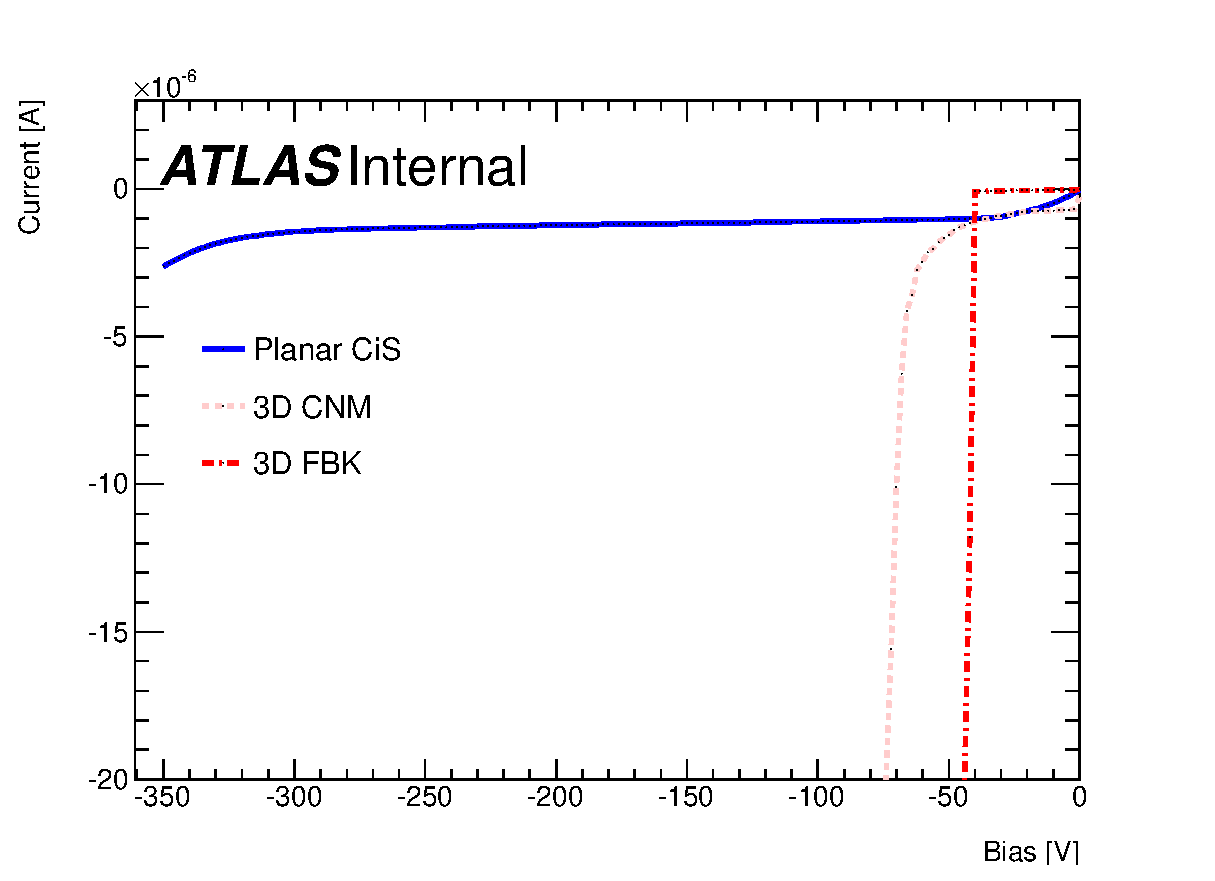
\includegraphics[width=6.7cm]{Images/ibl_stave_loading/ModuleReceptionTest/iv_alltec.eps}
%		\caption{Typical I-V behavior for Planar and 3D sensors. A current limit of $-20~\mu$ was used to protect the modules.}
%		\label{figure:ivmodules}
%	\end{subfigure}\quad
%       \begin{subfigure}[t]{0.4\textwidth}
%        		\centering
%                	\includegraphics[width=7cm]{Images/ibl_stave_loading/ModuleReceptionTest/S-Curve_Fit.png}
%                	\caption{Example of the S-Curve for one pixel, X axis shows the VCAL injection parameters and the conversion in electrons}
%                	\label{figure:SCurve}
%        \end{subfigure}\\
%        \begin{subfigure}[t]{0.4\textwidth}
%       		\centering
%               	\includegraphics[width=7cm]{Images/ibl_stave_loading/ModuleReceptionTest/thresh_alltec.png}
%                	\caption{Example of Threshold distribution for the IBL technologies. The distribution of the Planar sensors was the sum of the two FE-I4 contributions.}
%			\label{figure:ThresholdModules}
%	\end{subfigure}\quad
%        \begin{subfigure}[t]{0.4\textwidth}
%        		\centering
%                	\includegraphics[width=7cm]{Images/ibl_stave_loading/ModuleReceptionTest/noise_alltec.png}
%                	\caption{Example of Noise distribution for the IBL technologies. The distribution of the Planar sensors was the sum of the two FE-I4 contributions.}
%                	\label{figure:NoiseModules}
%        \end{subfigure}   	
        
%        \caption{Examples of electrical and functional tests performed at University of Geneva}
%        \label{fig:USBpixsetup}
%\end{figure}

%------------------------------------------
%\paragraph{Crosstalk scan}
%------------------------------------------
%In the crosstalk scan, the charge was injected in two neighbor pixels of the pixel under test, while the readout was enabled only for this one.
%Measurable crosstalk indicates excessive coupling, which can be caused by shorted bumps.
%Crosstalk scan allows to measure the crosstalk fraction and detect bump defects resulting in increased capacitive coupling between pixels. %(too large bumps, small separation between sensor and FE electronics, pouring of glue in the sensor-FE interstitial region)
%Because of capacitive or resistive coupling of the injected pixel with its neighbors, part of its charge can leak and be collected on the nearby channel.
%In this test the charge was injected in two over next pixels on the long pixel size, while only the pixel in between was enabled for readout.
%Usually it was not possible to inject large enough charges to see cross-talk hits using the on chip injection circuitry on depleted FE-I4 based modules, due to the limitation of the a maximum inject able charge of 55 %000 electrons. So measurable cross-talk indicates some excess coupling which can be caused by shorted or almost shorted bumps \cite{IBL-module-qualification}.
%Measurable cross-talk indicates some excess coupling which can be caused by shorted or almost shorted bumps \cite{IBL-module-qualification}.

%------------------------------------------
\paragraph{Tuning}
%------------------------------------------
The threshold and ToT response could be change acting on the following FE-I4 register:
\begin{itemize}
\item V$_{th}$, a 8-bit global register for the control of the threshold;
\item	TDAC, a 5-bit local register for the control of the threshold;
\item PrmpVbpf, a 8-bit global register for the control of the feedback current of the pre-amplifier;
\item FDAC, a 4-bit local register for the control of the feedback current of the pre-amplifier.
\end{itemize}
where a global register controls the entire pixel matrix and the local register controls a single pixel.
The optimization of the parameter required a dedicated tuning procedure. Since the level of the threshold affects the ToT response by definition, at least two iteration of tuning procedure were required. 
The tuning consisted in four main scan, each one dedicated to one register type, following the previous order. Each step consisted in a binary search across the register range of the target threshold or ToT.

\subsection{FE-I4 production and QA}
\label{sec:mod_electronic}
The production of the FE-I4 chip was carried out at IBM for a total of 3060 chips. Each FE-I4 had to pass a selection process testing the analog and digital functionality of each pixel, the global chip parameters and the chip calibration. The selection was based on the characterization performed on the first 600 chips.  A detailed description of the selection process can be found in \cite{WaferAnalysis}. In particular the FEs were accepted if less than \SI{0.2}{\percent} of the pixels were failing with less than 20 pixels per column. 
In total 61$\percent$ of the tested FE-I4 qualified for the IBL. The test results of the fully probed chips leading to a disqualification for IBL usage were shown in Figure~\ref{fig:failures}.
%
\begin{figure}
	\centering
		 \includegraphics[width=0.7\textwidth]{Images/ibl_paper/chapter04_Modules/failures.pdf}
	\caption{\textbf{}Failure modes leading to a disqualification of the FE-I4s for IBL operation. All 2814 fully probed chips were taken into account. Each bin shows the failure mode in percent. The bin \textit{Pixel matrix failures} indicatets FEs where the number of bad pixels were too high ($>$\SI{0.2}{\percent} failing pixels or $>$20 pixels per column). The bin \textit{Injection circuit failures} sums up all failures related to this circuit (low maximum voltage, injection delay not configurable, etc.). The bins \textit{High analog/digital current} combine current measurements at different chip states (unconfigured, configured, high digital activity). The next three bins give the rate for chips failing the global register tests, the reference current generation and the scan chain tests. All failure modes that were not explicitly mentioned contribute with only \SI{0.2}{\percent} and were summed up in the bin \textit{Else}. A total of 1,821 chips passed all tests giving a production yield of approximately \SI{60}{\percent}.}
\label{fig:failures}
\end{figure}
%
%Pixel failures lead to the disqualification of about \SI{25}{\percent} of the chips. About \SI{5}{\percent} of the FEs were disqualified due to failures in the internal injection circuit.
%To ensure the capability to calibrate the FE-I4 with the charge injection circuit during IBL operation rather strict cuts were applied here. Additional IDDQ\footnote{Measurement of the supply current (Idd) in the quiescent state.}, Scan chain and Shmoo plot\footnote{A plot showing the range of conditions (voltages, temperatures and inputs) in which the chip operates.} tests had been carried out at an external company for the first $\sim\,20$ wafers only, since the failure rate was low~($<$\SI{0.5}{\percent}).
%In total, \SI{60}{\percent} of the chips qualified for IBL. This number represents the overall production yield and had only limited significance for the process yield.



%For the IBL production, 3,060 FE-I4 chips on 51 \SI{200}{\milli\meter} wafers were tested and a complete list of the tests and a detailed description of the cut scheme can be found in~\cite{WaferAnalysis}.
%The data acquisition and handling was performed with the read-out system USBpix in combination with STControl%\footnote{version: trunk, rev. 8184}, a software application based on the ATLAS PixLib package~\cite{USBpix,Aad:2008zz}. A custom made PCB was designed to interface the read-out system hardware with a needle card, which establishes electrical contact with 108 FE pads. The steering of different scan routines, power supplies, multimeters, and the probe station was done by the read-out software allowing automated testing.
%All 60 chips of a wafer were probed with an average measurement time of ~2.5 days. The goal was to identify front-ends that were suitable for the IBL and measure calibration constants. 
An important step of the FE-I4 production was the chip calibration, because it can happen only at this stage. The chip calibration was carried out by using dedicated pads that cannot be bonded after the module assembly. No failing was allowed at the chip calibration stage.\\
The chip calibration consisted in the measurement of the voltage corresponding to the DAC of the pulser (PlsrDAC) and in the measurement of the injection capacitance. These two parameters allows to determine which charge was injected in the FEs circuitry with the injector. The calibration constants for the entire IBL production was shown in Figure~\ref{fig:calibration_results}.\\
The on-chip power regulators of the FE chips were not tested during the probing, but only after the modules had been assembled completely, see section~\ref{sec:module_qa}.

%
%%%% commented a' la Fabian
%\begin{figure}[h]
%	\centering
%	 \subfloat[][]{\label{fig:reference_current}\includegraphics[width=0.49\linewidth]{Images/ibl_paper/chapter04_Modules/PlsrDACslope.pdf}}
%	 \subfloat[][]{\label{fig:injection_capacitance}\includegraphics[width=0.49\linewidth]{Images/ibl_paper/chapter04_Modules/Injection_capacitance.pdf}}
%	\caption{\textbf{Calibration constants of the internal charge injection circuit}. The circuit distributes a voltage step to injection capacitors present in each pixel. (a) The slope of the transfer function of the voltage DAC~(\textit{PlsrDAC}). (b) The measured value of 3000 test injection capacitors present in each chip. On average the injected charge changes with the PlsrDAC setting: $\frac{\Delta Q}{\mathrm{DAC}} = 6.05\,\mathrm{fF} \cdot 1.45\,\frac{\mathrm{mV}}{\mathrm{DAC}} = 55\,\mathrm{e} / \mathrm{DAC}$.
%	}
%	\label{fig:calibration_results}
%\end{figure}

% using format as in chapter 6
\begin{figure}
	\centering
		\subfloat[\label{fig:reference_current}]{ \includegraphics[width=0.49\textwidth]{Images/ibl_paper/chapter04_Modules/PlsrDACslope.pdf}}
		 \subfloat[\label{fig:injection_capacitance}]{\includegraphics[width=0.49\textwidth]{Images/ibl_paper/chapter04_Modules/Injection_capacitance.pdf}}
  \caption{\textbf{}Calibration constants of the internal charge injection circuit. The circuit distributes a voltage step to injection capacitors present in each pixel. (a) The slope of the transfer function of the voltage DAC~(\textit{PlsrDAC}). (b) Distribution of measured values of almost 3,000 injection capacitors. On average the injected charge changes with the PlsrDAC setting: $\frac{\Delta Q}{\mathrm{DAC}} = 6.05\,\mathrm{fF} \cdot 1.45\,\frac{\mathrm{mV}}{\mathrm{DAC}} = 55\,\mathrm{e} / \mathrm{DAC}$.}
	\label{fig:calibration_results}
\end{figure}



%\noindent More than 50 different tests were used to evaluate the response to charge injection, the functionality of the digital hit processing periphery, the chip configurability, and the power consumption. About 18,000 values were recorded per wafer. WaferAnalysis, a custom made software designed for wafer and module tests of the IBL production, was used to determine the chip states automatically.
%The selection cut values were defined after the distributions of the first ten wafers had been studied.  8\% of the FE chips showed a anomalously high current at start-up and therefore were not fully probed. 


\subsection{Sensor Production}
%\paragraph{Production and QA}
\label{sec:sensor_qa}
\begin{figure}
\centering
\subfloat[\label{fig:planar_3D}]{\includegraphics[width=0.45\textwidth]{Images/ibl_paper/chapter04_Modules/Vbd_IBL.pdf}}
\subfloat[\label{fig:planar_after_dicing}]{\includegraphics[width=0.45\textwidth]{Images/ibl_paper/chapter04_Modules/Vbd_IBL_AfterDicing.pdf}}
\caption{The breakdown voltages of Planar  and FBK 3D sensors measured at the wafer level were presented in (a). The entry behind the vertical line indicates the Planar  sensors with breakdown voltage beyond \SI{200}{\volt}. The breakdown voltage of the Planar  sensors after under-bump metallization and dicing was shown in (b).}
\label{fig:sensor_breakdown}
\end{figure}

The Planar sensor production was carried out at CiS. A total of 150 wafers of Planar sensors were produced, each of them was four inch in diameter and \SI{200}{\micro\meter} thick and it hosted sensors, for an overall production of 600 sensors.
Each wafer was tested before the module assembly and it had to fulfill both electrical and metrology requirements.
The Planar  design includes a grid structure that allows biasing of the entire sensor by means of a punch-through technique.  This bias grid was used to evaluate the quality of the tiles at wafer level, before the dicing and the assembly to the FE-I4.
The sensors were polarized in reverse bias voltage, for sake of simplicity the voltage value will be reported in absolute value. The depletion voltage (V$_{dep}$) had to be in the range \SIrange{15}{75}{\volt} and current at the operative voltage (V$_{dep}$+\SI{30}) had not to exceed \SI{2}{\micro\ampere}. The ratio between the current at the operative voltage  and the current at the depletion voltage had to be lower then 1.6. The wafer thickness had to be in the range \SIrange{180}{220}{\micro \meter}, with a Planar ity lower than \SI{40}{\micro\meter}. A total number of 119 wafers was qualified, the rest of them was either damaged during the processing itself or it did not pass the selection criteria.\cite{Witting_thesis}\\
The 3D sensor production was carried out by two differente vendors, FBK and CNM. In total 118 wafer were produced, 58 at FBK and 60 at CNM. Each  wafer was 4 inches in diameter for a \SI{230}{\micro\meter} thickness.
For the testing, a different approach was used in the IV characterization, in particular it was difficult to implement a bias grid similar to the one used in Planar technology. FBK sensors used a temporary metal grid that was shorting all the pixel in the same column to a pad located in the periphery of the active region. The I-V curves of the 80 columns were measured with a probe card. The metal layer was removed before the dicing by chemical etching.\\
The depletion voltage had to be lower than \SI{15}{\volt} and the current at the operative voltage (V$_{dep}$+\SI{10}{\volt}) had not to exceed \SI{2}{\micro\ampere}. The ratio between the current at the operative voltage and the current at the depletion voltage had to be lower then 2. Wafers with 3 or more selected tiles were selected for the bump-bonding process and dicing.\cite{Nanni_3D}\\
The CNM sensor selection criteria were based on the leakage current measured through the 3D guard ring structure that surrounds the pixelated area. % While the p-side of the wafer was biased, the 3D guard ring was connected to ground via a dedicated pad, and the I-V curve measured for each sensor before the wafer was diced. After hybridization, the 3D guard ring was connected to ground through two special bumps of the FE-I4 chip.
The CNM sensors were required to had a breakdown voltage higher than \SI{25}{\volt}, the depletion voltage lower than \SI{15}{\volt}, and guard ring current lower than \SI{200}{\nano\ampere} at the operative voltage, which was set \SI{10}{\volt} above the depletion voltage. The ratio of the current in between the operative and the depletion voltage was also constrained to be less than 2. Wafers with at least 3 sensors that passed the selection criteria were sent to IZM for under-bump metallization and dicing.\cite{Nanni_3D}\\
During module assembly several CNM 3D modules showed a low breakdown voltage due to the poor correlation between the breakdown voltage measured on the wafer.
Initial studies indicated a good correlation between the breakdown voltage measured through the 3D guard ring structure and the breakdown voltage after detector assembly~\cite{IBL_mod_proto}.  However, during module assembly, the correlation proved to be poor, with several CNM 3D modules showing a low breakdown voltage. At this stage, all the sensors that were not assembled were re-tested on a probe station.  The n-side of the sensor was placed in contact with a grounded chuck via the under-bump metallization (see Section~\ref{sec:mod_bumping}), while the p-side was connected to the bias potential.  The sensors that showed a voltage breakdown larger than \SI{25}{\volt} were selected for hybridization. The yield of the CNM production on selected wafers as measured with the 3D guard ring method, was \SI{72}{\percent}.  However, after re-testing, the final production yield was similar to the FBK one.

% Planar 

% I_leak(Vdepl+30V)<2uA, slope=I_leak(Vdepl+30V)/I_leak(Vdepl)<1.6

%The leakage current of the Planar  tile, evaluated at the operative voltage (\SI{30}{\volt} above the depletion voltage), was required to be $\SI{<1}{\micro\ampere}$, and the ratio of the current for the operative and the depletion voltage needed to be lower than 1.6.  Wafers with two or more Planar  tiles that satisfied this requirement were sent for under-bump metallization and dicing at IZM.  The yield of the Planar  production, that was the percentage of Planar  tiles satisfying the above criteria, before under-bump metallization and dicing, was \SI{90.6}{\percent}. The breakdown voltage of the Planar  sensors was shown in Figure~\ref{fig:sensor_breakdown}. %% Ref Planar  yield: Witting, IBL GM 10 Oct 2012.


%\textbf\large{SG COMMENT:} \emph{Planar wafers with 2 good tiles were also counted (see Tobias 10 Oct 2012 IBL GM presentation.}\\

% 3D
%Due to the difficulty of implementing a bias grid structure compatible with the 3D design, alternative evaluation methods were developed for 3D sensors. FBK sensors included a metal grid that connected all the pixels in every column to a pad located in the periphery of the active region. Thus, by measuring the I-V curves of the 80 columns with a specially designed probe card, the quality of each sensor on the wafer was checked. The metal layer was removed before dicing by chemical etching, and the wafers with 3 or more selected tiles were sent to IZM for under-bump metallization and dicing. The sensors that passed the selection criteria were bump-bonded to read-out chips.

%The FBK sensors were required to had a breakdown voltage higher than \SI{25}{\volt}, a depletion voltage lower than \SI{15}{\volt}, and current at the operative voltage needed to be lower $\SI{2}{\micro\ampere}$, with the operational voltage \SI{10}{\volt} above the depletion voltage. The ratio of the current in between the operative and the depletion voltage was also constrained to be less than 2. The yield on the selected FBK wafers was \SI{57}{\percent}.  The breakdown voltage of the FBK 3D sensors measured before the wafers were diced was shown in Figure~\ref{fig:planar_3D}.

%The CNM sensor selection criteria were based on the leakage current measured through the 3D guard ring structure that surrounds the pixelated area. While the p-side of the wafer was biased, the 3D guard ring was connected to ground via a dedicated pad, and the I-V curve measured for each sensor before the wafer was diced. After hybridization, the 3D guard ring was connected to ground through two special bumps of the FE-I4 chip.

%The CNM sensors were required to had a breakdown voltage higher than \SI{25}{\volt}, the depletion voltage lower than \SI{15}{\volt}, and guard ring current lower than \SI{200}{\nano\ampere} at the operative voltage, which was set \SI{10}{\volt} above the depletion voltage. The ratio of the current in between the operative and the depletion voltage was also constrained to be less than 2. Wafers with at least 3 sensors that passed the selection criteria were sent to IZM for under-bump metallization and dicing.

%Initial studies indicated a good correlation between the breakdown voltage measured through the 3D guard ring structure and the breakdown voltage after detector assembly~\cite{IBL_mod_proto}.  However, during module assembly, the correlation proved to be poor, with several CNM 3D modules showing a low breakdown voltage. At this stage, all the sensors that were not assembled were re-tested on a probe station.  The n-side of the sensor was placed in contact with a grounded chuck via the under-bump metallization (see Section~\ref{sec:mod_bumping}), while the p-side was connected to the bias potential.  The sensors that showed a voltage breakdown larger than \SI{25}{\volt} were selected for hybridization. The yield of the CNM production on selected wafers as measured with the 3D guard ring method, was \SI{72}{\percent}.  However, after re-testing, the final production yield was similar to the FBK one.



\subsection{Module assembly and QA}
In this section a description of the module assembly and of the qualification performed on the modules was given.

\subsubsection{Module assembly}
\label{sec:mod_bumping}

%The connection between sensor and electronics was done by means of fine-pitch bump bonding and flip-chip technology. The read-out chip was thinned during bump-bonding to \SI{150}{\micro\meter}.% Only \SI{2}{\milli\meter} of the chip length or \SI{14}{\percent} of the chip area was dedicated to End-of-Column (EoC) logic outside the active area. Once bonded, most of these EoC part extends beyond the sensor area so that the wire bonding pads at the output of the EoC logic were still accessible to connect the read-out chip via aluminium-wire wedge bonding. Due to the design differences of the two sensor concepts the ratio of the active area with respect to the entire module area differs slightly between the two module types. For a Planar  double chip module, \SI{84}{\percent} of the module area was active, whereas \SI{80}{\percent} of the area for the 3D single chip modules was active.

%Fine pitch bump-bonding and flip-chip with the required pitch of \SI{50}{\micro\meter} had been successfully used for the construction of the ATLAS pixel detector modules~\cite{Aad:2008zz}. For the IBL modules an electroplated (SnAg) bumping process provided by IZM\footnote{Fraunhofer IZM, Gustav-Meyer-Allee 25, 13355 Berlin, Germany} had been used. 
The first step of the module construction consisted in the channel by channel connection of the sensor with the FE-I4, this operation was the bump-bonding process.
The bumping process was done at IZM\footnote{Fraunhofer IZM, Gustav-Meyer-Allee 25, 13355 Berlin, Germany} and it consisted  of the following steps.
\begin{itemize}
\item The FE-I4 thickness was reduced to \SI{150}{\micro\meter}.
\item Under-bump metallization: a metal stack of Ti/W and Cu was the sputtered on sensor and FE-I4 aluminum pads, which otherwise would not be solderable.
\item Deposition of the solder bumps on the FE-I4 wafer via electroplating technique.
\item Dicing of the sensor wafer and flip chip.
\item Bump soldering.
\end{itemize}

% This was divided into two steps: under-bump metallization (UBM) with solder bump deposition on the sensor and electronic wafers and flip chip of the diced FE-chips to the diced sensor tiles. The non-solderable aluminium pads of the sensors and read-out chips require an under-bump metallization for a reliable bump connection. The UBM metal stack, consisting of Ti/W and Cu, was sputtered on both sensor and read-out wafers. The solder bumps were only deposited to the read-out wafers using electroplating. The read-out wafers were thinned to the target chip thickness before UBM and bump deposition. After dicing of the sensor wafers the flip-chip process can be done. The read-out chip was placed on the sensor substrate with high accuracy and the assembly was soldered to form the electrical and mechanical interconnection between the pixel in a reflow soldering process.

Given the high temperature of the soldering process and the thin thickness of the IBL readout chip, a \SI{500}{\micro\meter} thick glass carrier chip was temporally mounted to the read-out chip and removed again after the reflow soldering. This prevents any deformation of the chip.
%For the IBL module production this process needed to be adapted for the large and thin read-out chips~\cite{thin-chip-bb-izm}. The roughly 2 by \SI{2}{\centi\meter\squared} FE-I4 chips thinned down to \SI{150}{\micro\meter} develop an unacceptable high deflection of more than \SI{40}{\micro\meter} during the high temperature reflow soldering leading to unconnected bumps especially in the outer areas of the assemblies. To avoid this chip deflection a \SI{500}{\micro\meter} thick glass carrier chip was temporally mounted to the read-out chip and removed again after the reflow soldering.
The glass was then removed by mean of a UV excimer laser with a wavelength of \SI{248}{\nano\meter}, the glass carrier material waswas optimized for the UV transmittance and the laser light was fully absorbed in the polyimide bonding layer.\\
%Mounting of the glass carrier was done on wafer level after thinning of the read-out wafers but before UBM and bump deposition. The entire stack of read-out wafer and glass carrier was diced prior to flip chip enabling the reinforcement of the glass carrier to the thin chip during the reflow soldering. But the high reflow temperatures of about \SI{250}{\celsius} requires a temperature stable wafer bonding technology together with an easy debonding capability at temperatures well below the reflow temperature. A polyimide bonding technique was chosen which allows for a laser induced debonding at room temperature of the glass carrier after flip chip. Thwas debonding process uses an UV excimer laser with a wavelength of \SI{248}{\nano\meter} exposed through the glass carrier to the bonding interface. The glass carrier material was optimised for the UV transmittance and the laser light was fully absorbed in the polyimide bonding layer. Above a certain level of energy fluence the material was decomposed and the bonding interface  was  opened so that the glass carriers can be easily removed from the backside of the read-out chips.
The first batches of module production showed a high bump-bonding failure rate due to large areas of disconnected bumps and isolated shorts between neighbor pixels.
The disassembled sensors and FE-chips of defective modules revealed polymerized flux residuals. The residuals acted as a spacer during the reflow preventing a proper bump connection between sensor and FE pixel. The disassembled modules revealed flux residuals in areas with larger number of shorts too, with the short vanishing after the disassembling. The flip-chip procedure was then changed, in particular the solder flux was replaced with glycerin.\cite{bump_bonding}
% As consequence of these findings IZM changed the flip chip procedure. The solder flux applied to the FE-chip prior to the flip chip and reflow was replaced with a glycerin as new tacking media. With this new flip chip method none of the problems were observed any more.

%\subsubsection{Module assembly}
%\label{sec:mod_assembly}
%Final module assembly was performed at the module production sites, at University of Genova and University of Bonn. 
The step following the bump-bonding procedure was the module dressing, which consisted  of the loading of the flex service and the wire-bonds connection for the FE and sensor pads. The module dressing consisted  in the following operation.
\begin{itemize}
\item Preparation and cleaning of the module flex hybrid, including visual inspection: here the flex hybrid was treated with special cleaning fluids\footnote{Vigon A200} in an ultrasonic bath. % and afterwards rinsed with warm and purified water to remove any remnants of the cleaning fluid.
\item Preparation and visual inspection of the bare module.
\item Aligning of the module flex hybrid to the module, depositing of the glue and curing.
\item Activation of the wire-bonds pads via plasma cleaning.
\item Wire bonding of the FE-chip to module flex hybrid and of the wire bond bridge to the test connector.
\end{itemize}

%Both module production sites had very similar assembly procedures but the assembly procedure may differ in some details between the two sites. After visual inspection the module flex hybrid electric test was repeated.
%The first step of the assembly procedure was the preparation and cleaning of the module flex, which was required for. 
%The flex hybrid was treated with special cleaning fluids (Vigon A200) in an ultrasonic bath and afterwards rinsed with warm and purified water to remove any remnants of the cleaning fluid. Finally it was dried in an oven and the wire bond pads were activated via plasma cleaning.

%The second step was the visual inspection of the bare module, in particular checking for scratches and damages. %The bare module was carefully inspected, particularly for scratches and other damages. For the Planar  DC modules an I-V measurement was performed to ensure the sensor quality after flip chip. Finally the bare module was weighted and the data were stored for later reference. 
%Next step was the positioning of the bare module and module flex on the assembly tool by aligning them to the alignment marks of the tool. Two types of glue were used: a double tape strip (PPI RD-577F) underneath the FE-I4 wire bond pads and an epoxy glue (UHU EF 300 or Araldite 2011) underneath the remainder of the flexes. Pressure was applied on the critical wire bond regions during curing to ensure a sufficient flatness of the pads for wire bonding.

%Final step of the assembly was the wire bonding of the FE chip and sensor to the flex and the intermediate wire bond bridge of the module flex. Both bondings were performed with \SI{25}{\micro\meter} thick aluminium wires on a fully-automated wire bond machine. For all modules ten to twenty bonds of both areas were pulled and the pull forces were stored to monitor the wire bond quality. Each assembly step was documented to a traveller which follows the module during all the production steps. At the end of the assembly the module was visually inspected in detail and any inconsistency was written to the module traveller.

\begin{figure}
	\centering

		\subfloat[\label{fig:SC_picture}]{		 \includegraphics[width=0.335\textwidth,angle=180]{Images/ibl_paper/chapter04_Modules/IBL_module_photo_SC_HD.jpg}}
		\subfloat[\label{fig:DC_picture}]{ \includegraphics[width=0.655\textwidth,angle=180]{Images/ibl_paper/chapter04_Modules/IBL_module_photo_DC_HD.jpg}}
  \caption{Photographs of a dressed IBL single chip module (a) and a double chip module (b). The flex extension visible on the top allows testing of the module before loading on stave. It was cut during the stave loading procedure at a cutting line slightly above the bare module.}
	\label{fig:module_pictures}
\end{figure}


\subsubsection{Module QA }
The modules underwent through a QA which included tests of the electrical and functional performance of both FE-I4 and sensors. This characterization was performed at room temperature and at \SI{-15}{\celsius}, the latter in order to test the module in the environmental condition of the expected IBL operation.
During the module QA the power regulators were tested for the first time and also calibrated, digital and analog circuitries of the FE-I4 were as well tested. An aging tests was performed as well, this consisted of ten thermal cycles of the module in \SIrange{-40}{40}{\celsius}, in which the module was not operative. 
A detailed description of the module QA and chip calibration can be found in \cite{Malte_thesis}, the module selection for the stave loading was done according to the results of these performance tests. Only modules passing all tests were considered as candidates for IBL. The number of failing pixel of each test was summed up without counting pixel twice if they were failing more than one test. For any module, nonconformities like rework, sensor scratches or chip chipping penalties in terms of additional bad pixels were put in the bad pixel count. Only modules with a total number of bad pixel count below \SI{1}{\percent} were selected. This means, for double (single) chip modules, less than 540 (270) bad pixels were tolerated.\\
Of particular interests for this work of thesis was the characterization of module performance in terms of the sensor breakdown voltage, the fraction of failing pixels and the timing performance of modules production. In particular the breakdown voltage and the fraction of failing pixels were used for determining the position of the module into the stave, while the timing performance became crucial in the commissioning phase of the detector.\\
\begin{figure}
	\centering
		%\subfloat[\label{fig:SourceOcc}]
		 %{\includegraphics[width=0.49\textwidth]{Images/ibl_paper/chapter04_Modules/Source_Occ_int.pdf}}
		%\subfloat[\label{fig:SourceSpectrum}]
		 %{\includegraphics[width=0.49\textwidth]{Images/ibl_paper/chapter04_Modules/Source_TOT_int.pdf}}
		\subfloat[\label{fig:VbdLogY}]{\includegraphics[width=0.49\textwidth]{Images/ibl_paper/chapter04_Modules/VbdDistLogY.pdf}}
		\subfloat[\label{fig:modTotalPixFail}]{}\includegraphics[width=0.49\textwidth]{Images/ibl_paper/chapter04_Modules/TotalPixFailLogY_int.pdf}
  \caption{(a) The dashed vertical line indicates the maximum measurement point of \SI{-400}{\volt} for the Planar  modules and the dotted vertical line the maximum measurement point of \SI{-120}{\volt} for the 3D CNM and FBK modules. Additionally, the acceptance criteria for the Planar modules above \SI{-150}{\volt} (green) and \SI{-150}{\volt} (red) were indicated by the shaded areas. The mean value of the distribution of 313 Planar  sensors was \SI{-375}{\volt}. The 3D CNM distribution of 128 CNM sensors had a mean value of \SI{-73}{\volt}. The distribution of 93 FBK sensors shows a mean value of \SI{-43}{\volt}. A percentage of 0.42 modules fails the indicated minimum acceptance level for Planar  and 3D CNM and FBK sensors. (b)The distribution of the fraction of pixels failing in any test. Only the accepted modules were taken into account. A pixel was considered as failing if it fails any one of the tests as described in the text.}
\end{figure}
The breakdown voltage differs for all three module flavours (Figure \ref{fig:VbdLogY}). The operation voltage of the two 3D module types was \SI{-20}{\volt}, hence all 3D modules with a breakdown voltage below \SI{-30}{\volt} were rejected. The sensor test procedure at wafer level was significantly different for the CNM and the FBK modules as explained in section~\ref{sec:sensor_qa}.
%An additional process step was used on the FBK modules to qualify the sensors at wafer level. A metal layer was applied to connect the pixel implants to GND, before the sensor was tested. After the test this metal grid was removed as this connection would be a short to all pixels. The CNM sensor characteristics was tested at wafer level using the guard ring as GND contact. The drawback of this method was the insensitivity to failures in the pixel array.
As a consequence, the correlation between the breakdown voltage measurement at wafer level and on dressed modules was poor for CNM modules. This was the reason for the increased number of dressed modules failing the minimum breakdown voltage cut of the CNM compared to the FBK modules. Additionally, the value of the measured current was dominated by surface current effects on the sensor. This makes the breakdown voltage determination difficult and thus the distribution broader than for the FBK modules. The dominance of the surface current was expected to disappear with the increased leakage current due to radiation damage in the silicon bulk.
The Planar  modules fulfill the cut criteria if there was a difference of more than \SI{70}{\volt} between the breakdown voltage and the operational voltage of \SI{80}{\volt}. All dressed modules with a Planar  sensor, but four, fulfill the sensor breakdown voltage criteria.
After the test of each individual failure mode, pixel failing any test were counted. Individual pixels were not double counted. %because most of the test routines were mutually dependent on each other. For example, a digitally unresponsive pixel fails in all other tests that require the detection of charges. 
The fraction of pixel that fails in any test was shown in Figure \ref{fig:modTotalPixFail} for all modules. The mean number of failing pixels of the accepted Planar  modules was about \SI{0.56}{\percent}. The distribution width was approximately \SI{1.67}{\percent}. As expected, the fraction of failing pixels distribution of the CNM and FBK modules was comparable to the Planar  module distribution with a mean of about \SI{0.52}{\percent} and an RMS of \SI{0.44}{\percent} in the CNM case and \SI{0.68}{\percent} mean and \SI{0.39}{\percent} RMS in the FBK case. 

\label{sec:module_qa}
\begin{figure}
\centering
    %\subfloat[\label{fig:T0_Scan}]{ \includegraphics[width=0.49\textwidth]{Images/ibl_paper/chapter04_Modules/T0_Scan_int.pdf}}
    \subfloat[\label{fig:TimewalkMeasure}]{\includegraphics[width=0.49\textwidth]{Images/ibl_paper/chapter04_Modules/Timewalk_measure_int.pdf}}
    \subfloat[\label{fig:OverdriveLogY}]{\includegraphics[width=0.49\textwidth]{Images/ibl_paper/chapter04_Modules/OverdriveDistPixelLogY_int.pdf}}
    \caption{\textbf{}(a) The pixel to pixel distribution of the in-time threshold and (b) the charge above the discriminator threshold this was needed for the hit to be detected within one bunch crossing. All modules matching IBL quality criteria were shown. The overdrive was measured after tuning the modules to \SI{3000}{\e} threshold and 10 ToT counts for a charge injection of \SI{16}{\kilo\e} at approximately -\SI{15}{\celsius}. The mean in-time threshold value of the Planar Normal (Long) distribution was \SI{3354}{\e} (\SI{3372}{\e}) with a RMS of \SI{313}{\e} (\SI{400}{\e}).% and 14,257,152 (365,568) entries.
The 3D CNM distribution had a mean value of \SI{3519}{\e} and a RMS of \SI{357}{\e}. %3D CNM had 2,661,120 entries. 
The 3D FBK distribution mean value was \SI{3820}{\e}, the RMS was \SI{483}{\e}.% and the number of entries was 2,204,160. 
Pixels failing the measurement were not included in the distributions.}
    \label{fig:modules:Timing_Scans}
\end{figure}

During the detector operation, IBL modules will be read using only a one bunch-crossing-wide Level-1 trigger. This mode translates to a sensitive time of only \SI{25}{\nano\second}. Thus the hit timing was of major importance for the IBL operation.% In order to measure the hit detection time using the on-chip charge injection circuitry, the charge injection time needs to be precisely measured and adjusted. For this
%The FE-I4 had an adjustable on-chip injection delay circuitry, which was used to tune the charge injection timing. 
%This circuitry adjusts the injection timing globally and therefore the injection delay must be adjusted in a scan algorithm for the whole chip. This scan measures the hit detection probability as a function of the delay setting for a large injected charge and one bunch crossing read-out. This results in a box-shaped function, as presented in Figure \ref{fig:T0_Scan}. The detection turn-on time was defined by the 50\,\% hit detection probability. The difference between detection turn-off time and detection turn-on time was known to be \SI{25}{\nano\second} and this was used by an automated algorithm to calibrate the step-width of the delay circuitry. The step-width of this particular FE-I4 was approximately \SI{0.58}{\nano\second}.
The mean turn-on time of the full pixel array was measured and the injection time ($t_0$) was fixed to the mean turn-on time plus a safety margin of \SI{5}{\nano\second}.\\
Measuring the $t_0$ time as a function of the injected charge reveals the time-walk effect: the smaller the injected charge, the earlier the $t_0$ was measured and this could led a charge to be measured in the previous bunch crossing.
%The time-walk can be expressed in electrons and was defined as the charge above the discriminator threshold, at which the $t_0^{tw}$ was measured within the same bunch crossing as the $t_0$ at the maximum charge. Thus, the $t_0^{tw}$ was defined to $t_0$ minus \SI{20}{\nano\second}. 
A useful quantity for the characterization of the time-walk was the overdrive, the charge above the discriminator threshold that was needed for the hit to be detected within one bunch crossing. All hits with a charge above the discriminator threshold plus the overdrive will be detected within the same bunch crossing. This threshold was commonly called in-time threshold. 
The overdrive distribution of the Planar  modules (\SI{355}{\e} mean with a RMS of \SI{250}{\e}) was lower than the distribution of the CNM modules (\SI{530}{\e} mean with \SI{351}{\e} RMS), while the FBK modules had the highest overdrive (\SI{828}{\e} mean \SI{478}{\e} RMS). These time-walk values were well-below the time-walk correction capability of the read-out chip (approximately \SI{1500}{\e}, see~\cite{BackhausPhd}).\\
%The in-time threshold can also be conveniently measured using the normal threshold scan algorithm with a single Level-1 trigger read-out after careful $t_0$ adjustment beforehand. Therefore, the time-walk was measured during the IBL module production using the so-called overdrive (calculated as pixel-by-pixel difference of in-time threshold and the discriminator threshold taken from a standard threshold measurement). The in-time threshold as well as the overdrive distribution were given in Figure \ref{fig:modTimewalk}. The in-time threshold distributions show the expected influence of the sensor type. The detector capacitance influences the rise-time of the preamplifier and thus the time-walk. Similar to the noise distributions for the three module types, the overdrive distribution of the Planar  modules (\SI{355}{\e} mean with a RMS of \SI{250}{\e}) was lower than the distribution of the CNM modules (\SI{530}{\e} mean with \SI{351}{\e} RMS), while the FBK modules had the highest overdrive (\SI{828}{\e} mean \SI{478}{\e} RMS). These time-walk values were well-below the time-walk correction capability of the read-out chip (approximately \SI{1500}{\e}, see~\cite{BackhausPhd}).\\
%The limited available analog hit information due to the low number of ToT bits complicates the ToT to charge calibration. The simple conversion measurement used on the current ATLAS pixel modules (explained in detail in \cite{GKHabil}) measures a ToT histogram at pixel level as a function of the injected charge. The result was then used to fit a conversion function. This method does not result in a satisfactory ToT-to-charge calibration using FE-I4 based modules due to the few ToT bins.\\

%\begin{figure}[t]
%	\centering
%		\subfloat[\label{fig:TOT_LUT}]
%		{\includegraphics[width=0.49\textwidth]{Images/ibl_paper/chapter04_Modules/TOT_Calib_LUT_int.pdf}}
%		\subfloat[\label{fig:ChargeCalibration}]
%		{ \includegraphics[width=0.49\textwidth]{Images/ibl_paper/chapter04_Modules/PulserMean_vs_TOT_int.pdf}}
 % \caption{\textbf{}ToT to charge calibration. The mean and sigma of the pixel-to-pixel charge distributions were in shown (a). The charge calibration
%  function was depicted in (b).}
%	\label{fig:modToTCal}
%\end{figure}
%
%A new calibration method was implemented that measures injected charge histograms for each ToT. For each pixel the injected charge value was stored for the pixel that responds with the chosen ToT. This results in a charge histogram as shown in Figure \ref{fig:TOT_LUT}. The mean value and the width of the injected charge distributions were used as a look-up table for the ToT-to-charge calibration (see Figure \ref{fig:ChargeCalibration}). This new procedure benefits from the smaller step width of the injection circuitry (in terms of injected charge) in comparison with the large charge steps of the ToT information. This measurement was performed on each IBL module and the result was stored for each individual pixel.


%The source scan performed on each IBL module targets the measurement of the bump connectivity and not the charge calibration. The individual ToT information per pixel was not stored to limit the amount of recorded data. As a consequence, here the ToT-to-charge conversion was averaged over the entire chip. An example source scan result of a single chip was presented in Figure~\ref{fig:SourceOcc}.\\
%
%The leakage current as a function of the sensor bias voltage was measured at both quick operation and full performance test stage. The breakdown voltage was used to qualify the modules in this test. An example IV characteristic of ten randomly chosen modules was shown in Figure \ref{fig:IVten}. From these curves the breakdown voltage was extracted by a dedicated algorithm.
%


%Several scans were performed to reveal the bump failures at pixel level. These were threshold measurements without sensor bias applied, crosstalk measurements and source measurements. Several algorithms based on individual pixel hit number with respect to the average hit rate per pixel were implemented to identify the bump failure mode, either shorted (or with high coupling) or open bumps, in each tests and for different module types. A $^{241}$Am source scan occupancy was the most reliable test and thus was used for the final open bump detection.% In Figure \ref{fig:modSourceFail} the module distribution of the fraction of pixel failing the source test was shown. Pixels with less than \SI{5}{\percent} or more than \SI{450}{\percent} of the mean pixel occupancy were considered as failing. In total only a number of 19 modules had more than \SI{1}{\percent} bad pixel.

%\begin{figure}[htbp]
%	\centering
%		\subfloat[\label{fig:SourceLinY}]
%		 {\includegraphics[width=0.49\textwidth]{Images/ibl_paper/chapter04_Modules/SourcePixFail_int.pdf}}
%		\subfloat[\label{fig:SourceLogY}]
%		 {\includegraphics[width=0.49\textwidth]{Images/ibl_paper/chapter04_Modules/SourcePixFailLogY_int.pdf}}
 % \caption{\textbf{}The distribution of the fraction of pixels failing the occupancy criteria in the $^{241}$Am source scan in (a) linear scale and in (b) logarithmic scale. Only the accepted modules were taken into account. A pixel was considered as failing if it had less than \SI{5}{\percent} or more than \SI{450}{\percent} of the mean pixel occupancy.}
%	\label{fig:modSourceFail}
%\end{figure}





\subsubsection{Production Yield}
\label{sec:prod_yield}

%Module production for the IBL started in the second-half of 2012 and lasted until April 2014. Bare modules after flip chip and laser de-bonding of the glass carrier were delivered in batches of about twenty modules of different type, i.e. double chip modules with Planar  sensors and single chip modules made of 3D sensor from both vendors FBK and CNM. Modules were assembled at both module production sites and tested in detail as described in the previous section. After analysing the module test results, the modules were selected according to the acceptance criteria. Modules passing the criteria were sent to the next integration step which was the loading on staves as described in section~\ref{sec:stave_loading}. To ensure a sufficient supply of all types of IBL modules the entire module production and testing chain was organised for parallel processing of double chip and single chip modules.

% The later effect was illustrated in Figure~\ref{fig:module_shorted_bumps}.
%\begin{figure}[t]
%	\centering
%		 \includegraphics[width=0.8\textwidth]{Images/ibl_paper/chapter04_Modules/CrosstalkAnalogOverlay_int.pdf}
%	\caption{Measurement of the shorted bump effect for a double chip module of the first batch of IBL module production. Pixels failing the analog injection test were marked red. Pixel failing the cross-talk test were marked in blue. For nearly every pixel showing a high cross-talk a direct neighbour was failing the analog injection test suggesting that a low impedance electrical connection exists between the bumps.}
%\label{fig:module_shorted_bumps}
%\end{figure}
%The figure shows a combination of results of two standard tests. The first test was an injection of 200 test pulses into every pixel of the module. All pixels showing more or less hits were marked in red. The second test was a so-called cross-talk scan. During the cross-talk scan high test pulses of the order of \SI{50,000}{\e} were injected in both neighbours of each pixel per column. If the pixel in the middle detects any hit it was marked in blue. In this particular example almost all pixels showing cross-talk had a maximum cross-talk meaning that every injection into the neighbour pixel showed up in the read-out pixel. Conversely, the pixel failing the analog injection test fails completely, i.e. none of the 200 injections were detected in the pixel. Since for nearly every analog failing pixel a high cross-talk can be found in one of the direct neighbour pixel there must be a low impedance connection between the two pixels. Such an electrical connection between these two preamplifiers of the pixel will bring one of the preamplifier into saturation and therefore all the hits of the two shorted pixel were detected by the pixel connected to the amplifier still operational.

%During the production stop both bump defects were investigated in detail in close collaboration with IZM. These investigations included a careful evaluation of each step of the module production at IZM and the assembly sites as well as the disassembly of defective modules to investigate the origin of the defects. Both bump problems could be traced back to the usage of a flux during the soldering process. 
\begin{figure}
	\centering
		 \includegraphics[width=0.8\textwidth]{Images/ibl_paper/chapter04_Modules/ModuleProductionYield_Combined.pdf}
	\caption{\textbf{}Yield of IBL module production for sensor types of Planar (PPS) and 3D (CNM, FBK) per production batch group. In the top panel for failure modules,  \textit{B.B. Fail.} designates large bump-bonding failure,  \textit{Bare Fail.} for the modules not assembled due to mainly mechanical damages, and \textit{Other Fails.} were both electrical and sensor failures discovered after assembly. Within the same batch group, similar configuration of the laser vendor and the bump bonding was applied. In the bottom panel, the first batch group was excluded from the average yield in the plot because they were largely affected by bump bonding problems that were fixed in the following batches. The total average bad module fraction of all batches for PPS, CNM, FBK was 0.36, 0.50, 0.44, respectively.}
\label{fig:module_yield}
\end{figure}

Figure~\ref{fig:module_yield} summarizes the IBL module production yield. In the figure the yield was expressed in terms of bad modules and distinguishes between the three different types of IBL modules: Planar  modules were noted as PPS, 3D modules were from CNM and from FBK. The yield was divided into different production batches with similar laser de-bonding and flip chip method applied. % For instance all modules assembled with the initial flip chip method using the solder flux were grouped in L1 for all module types. Another important difference of the module assembly during the production time was connected with the laser de-bonding of the glass carrier. The initial vendor for the production turned out to be unreliable in terms of processing time so IZM had to qualify another vendor during the production. The first modules from this second vendor can be found in batch L3 for PPS and L4 for the FBK and CNM modules.

The production yield of the first batch group L1 of all modules was very poor due to the problems with the bump bonding.\cite{IZM_bonding} Only 40~\% of the Planar  modules, \SI{20}{\percent} of the CNM and \SI{35}{\percent} for the FBK 3D modules passed the acceptance criteria. For the other batches the yield improved to an average of \SI{75}{\percent} for the Planar  modules, \SI{63}{\percent} for CNM and \SI{62}{\percent} for FBK modules. % Only the initial modules coming from the second laser de-bonding vendor showed a significant higher rate of bump-bonding defects. This was mainly due to problems with the handling of the thin modules during and after the glass carrier removal. The bump defect rate for all other batches remained constant and was far below \SI{10}{\percent} for Planar  and CNM modules but was slightly higher (\SI{15}{\percent}) for FBK modules. 
Other main defects observed during the module production were either of mechanical or electrical origin. During the entire production a roughly constant defect rate of about 15 to \SI{20}{\percent} was observed which included all kind of electrical failures. Main contributions were failures of the on-chip regulators which were not tested during wafer probing of the read-out chip wafers. Also other electrical problems appeared, such as failing double columns of the FE and communications issues but the rates were quite low so no special effort was applied to improve this. A number of CNM modules in L2 and L3 showed problems with low breakdown behavior of the sensor. The reason for this was a insufficient testing procedure during the sensor wafer quality insurance. CNM sensors used for the batches L4 and L5 were retested after under bump metallization deposition and dicing and therefore the yield improved slightly. However, re-testing required the removal of the sensor from the clean room environment and the placing of the sensor pixel side to a metal chuck. Thus the additional dust and scratches were introduced which could not be cleaned properly prior to the flip chip. Therefore the bump bonding failure rate was increased for these batches with respect to the previous batches.\\

%The IBL module production was driven by the tight schedule of the IBL project. Main focus was the production of a sufficient number of good modules in time to feed the stave loading process. The total number of needed modules were relatively small as compared to the earlier ATLAS pixel module production. Thus even a relatively low production yield was accepted since improving the yield would had needed much more time than it was available for completing the IBL on schedule.


\subsection{Bare stave and flex assembly}
%\subsubsection{Stave flex gluing}
%A pair of  stave flexes was directly glued on the stave back stiffener. The attachment method was selected to match the stave envelop constraints, the required assembly accuracy (\SI{\pm0.3}{\milli\meter} in the longitudinal direction, \SI{\pm0.1}{\milli\meter} in the transverse direction), the radiation hardness (\SI{250}{\mega\radian}),  the thermo-mechanical constraints between two different material types and  the minimization of the material budget.\\
%After an intensive test campaign to validate the deposition process, the radiation, and the mechanical stiffness, the Araldite 2011 accompanied by a Kapton wet etching process for the flex surface were selected. Surface treatment of pyralux bondply LF111 as the flex bottom layer had been added in order to apply the glue directly to a \SI{25}{\micro\meter} acrylic layer and to avoid the Kapton gluing. The final validation
%was realised through a ageing tests with a production IBL stave glued with production flexes according to the final gluing procedure. Both thermal and radiation loads were applied to the assembly during the test at Ionisos Company (France) while using a \SI{10}{\mega\ev} electron source.
%After having been irradiated at about \SI{380}{\mega\radian} and thermally cycled 110 times between \SI{+40}{\celsius} and \SI{-40}{\celsius}, no critical damages were observed on the stave-flex glue joint~\cite{IrradiationStaveNote}. 

%Specific tools were used to allow precise glue deposition, see Figure~\ref{fig:FlexStaveGluing}, to align both parts and guaranty glue thicknesses.
%The assembly workflow was summarised  in Table~\ref{tab:FlexGluingWorkflow} and was executed in CERN Atlas cleanroom.
The assembly of the stave with the flex assembly was entirely performed in clean room. A visual inspection was performed as soon as the components were received from the respective production sites, each component was cleaned to prevent contamination of the flex services and the stave surfaces. Before the loading, an electrical test was performed on the flex, which had to stand \SI{1000}{\volt} for the HV lines dedicated to Planar modules and \SI{500}{\volt} for the HV lines dedicated to the 3D ones. The resistivity measurements indicated a value compatible with the \SI{0.196}{\ohm} one that was foreseen at the design.
After this electrical test the wings were bent and a second electrical test was performed. The flex was then loaded on the stave, glueing it to one of the stave back side. After the hardening of the glue the stave joints were checked with an endoscope. The stave was then loaded on dedicated designed handling frame and final glueing steps performed, which involved the carbon fibre clamping.
\begin{table}
        \resizebox{0.9\textwidth}{!}{\begin{minipage}{\textwidth}
        \begin{tabular}{|l|c|c|c|c|c|c|c|c|}
                \cline{2-9}
                \multicolumn{1}{r|}{}  & stave 1 & stave 2 & stave 3 & stave 4 & stave 5 & stave 6 & stave 7 & stave 8 \\
                \hline
                planarity   before [\SI{}{\micro\meter}]  & 218 & 178 & 176 & 217 & 108 & 219 & 177 & 157  \\
                planarity   after [\SI{}{\micro\meter}]   & 244 & 205 & 223 & 235 & 189 & 290 & 222 & 193  \\
                Dif. [\SI{}{\micro\meter}]   & 26 & 27 & 47 & 18 & 81 & 71 & 45 & 36  \\
                \hline
                \cline{2-9}
                \multicolumn{1}{r|}{}  & stave 9 & stave 10 & stave 11 & stave 12 & stave 13 & stave 14 & stave 15 & stave 16 \\
                \hline
                planarity   before [\SI{}{\micro\meter}]  & 195 & 194 & 230 & 280 & 186 & 181 & 135 & 283  \\
                planarity   after [\SI{}{\micro\meter}]   & 229 & 243 & 298 & 314 & 224 & 218 & 325 & 329 \\
                Dif. [\SI{}{\micro\meter}]   & 34 & 49 & 68 & 34 & 38 & 37 & 190 & 46  \\
                \hline
                \cline{2-5}
                \multicolumn{1}{r|}{}  & stave 17 & stave 18 & stave 19 & stave 20 & \multicolumn{1}{r}{} & \multicolumn{1}{r}{} &                      \multicolumn{1}{r}{} & \multicolumn{1}{r}{} \\
                \cline{1-5}
                planarity   before [\SI{}{\micro\meter}]  & - & 282 & 220 & 257& \multicolumn{1}{r}{} & \multicolumn{1}{r}{} & \multicolumn{1}{r}{} & \multicolumn{1}{r}{} \\
                planarity   after [\SI{}{\micro\meter}]   & 114 & 336 & 266 & 237 & \multicolumn{1}{r}{} & \multicolumn{1}{r}{} & \multicolumn{1}{r}{} & \multicolumn{1}{r}{} \\
                Dif. [\SI{}{\micro\meter}]   & - & 54 & 46 & -20 & \multicolumn{1}{r}{} & \multicolumn{1}{r}{} & \multicolumn{1}{r}{} & \multicolumn{1}{r}{} \\
                \cline{1-5}
        \end{tabular}
        \caption[Table caption text]{Production staves Planar ity before and after thermal cycle.}
        \label{table:planarity}
        \end{minipage} }
\end{table}





\begin{figure}
        \centering
        \subfloat[\label{}]{ \includegraphics[width=0.35\textwidth]{Images/IBL_Paper/chapter06_LoadingQA/Phi_0.pdf}}
        \subfloat[\label{}]{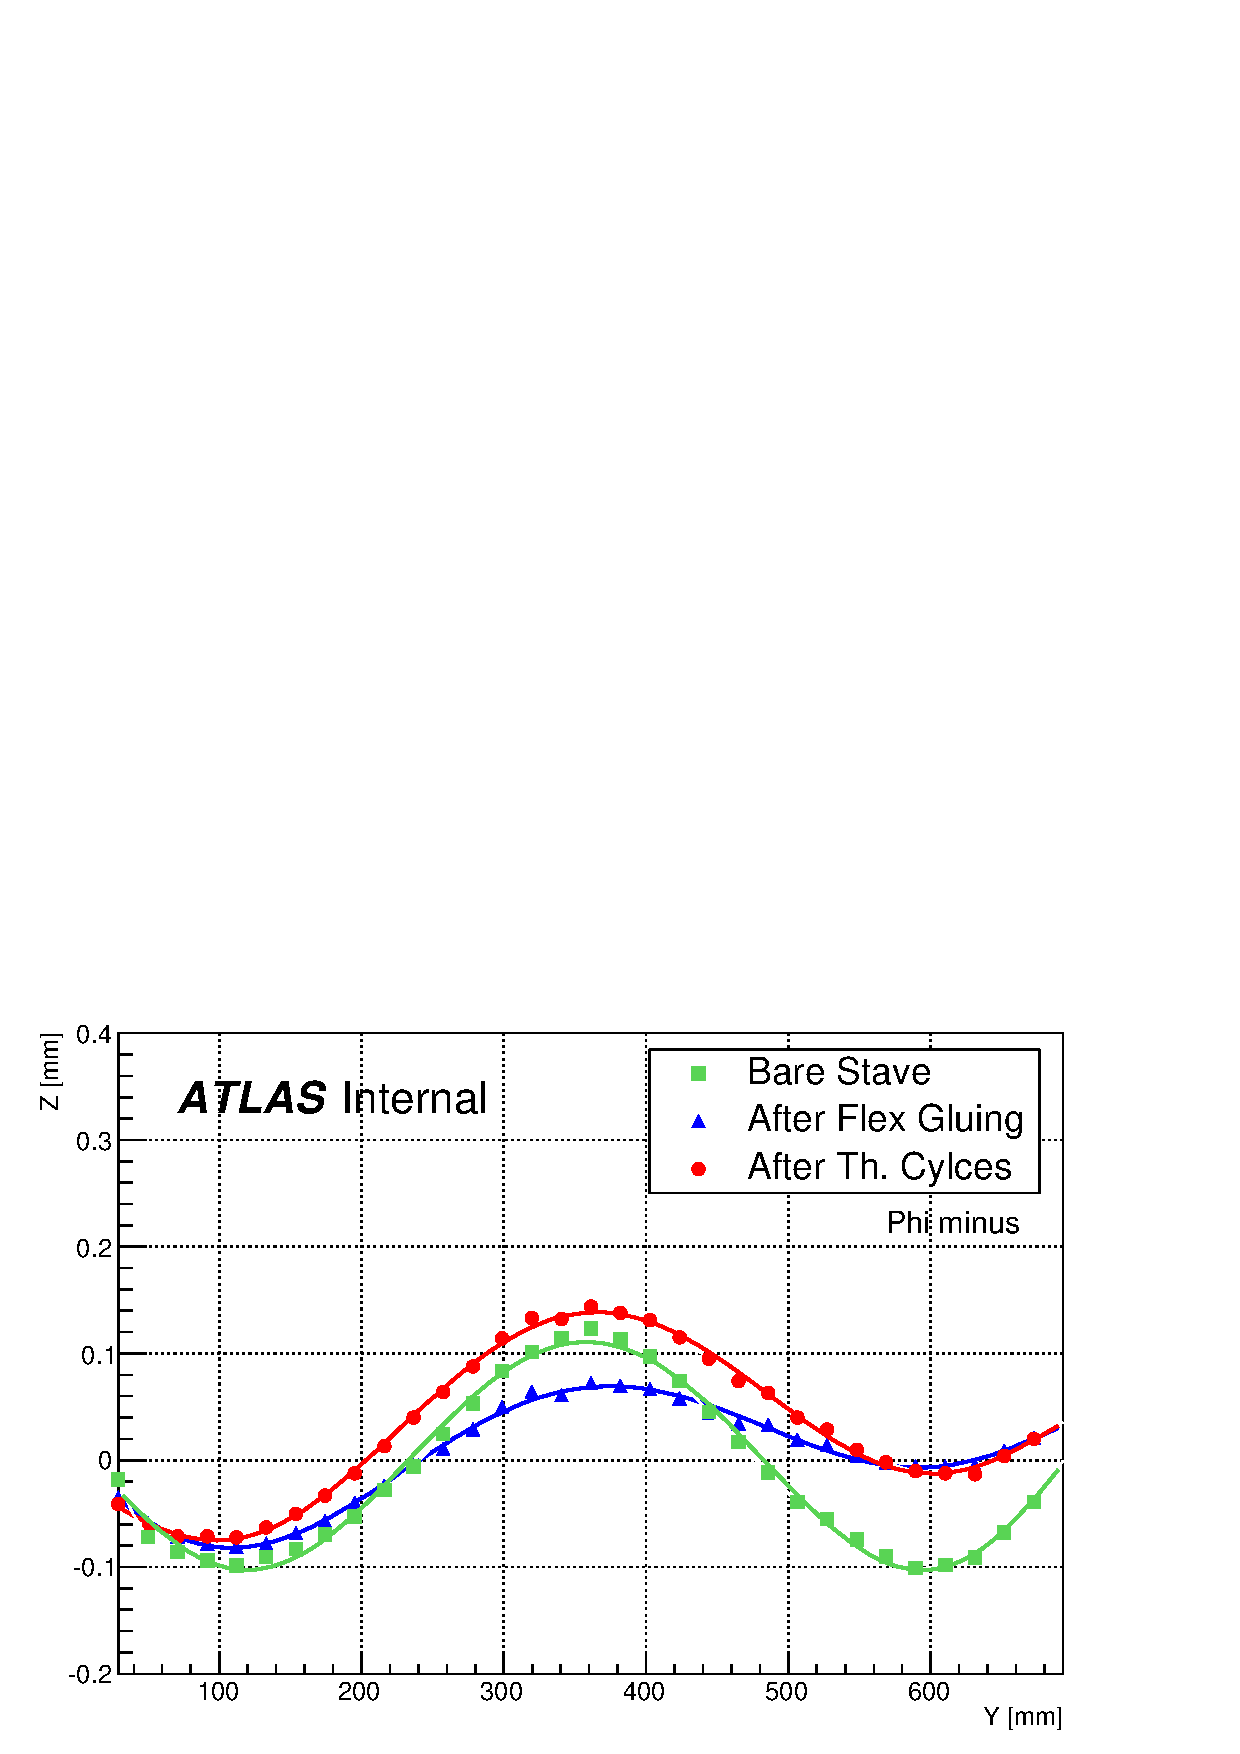
\includegraphics[width=0.35\textwidth]{Images/IBL_Paper/chapter06_LoadingQA/Phi_minus.pdf}}
        \subfloat[\label{}]{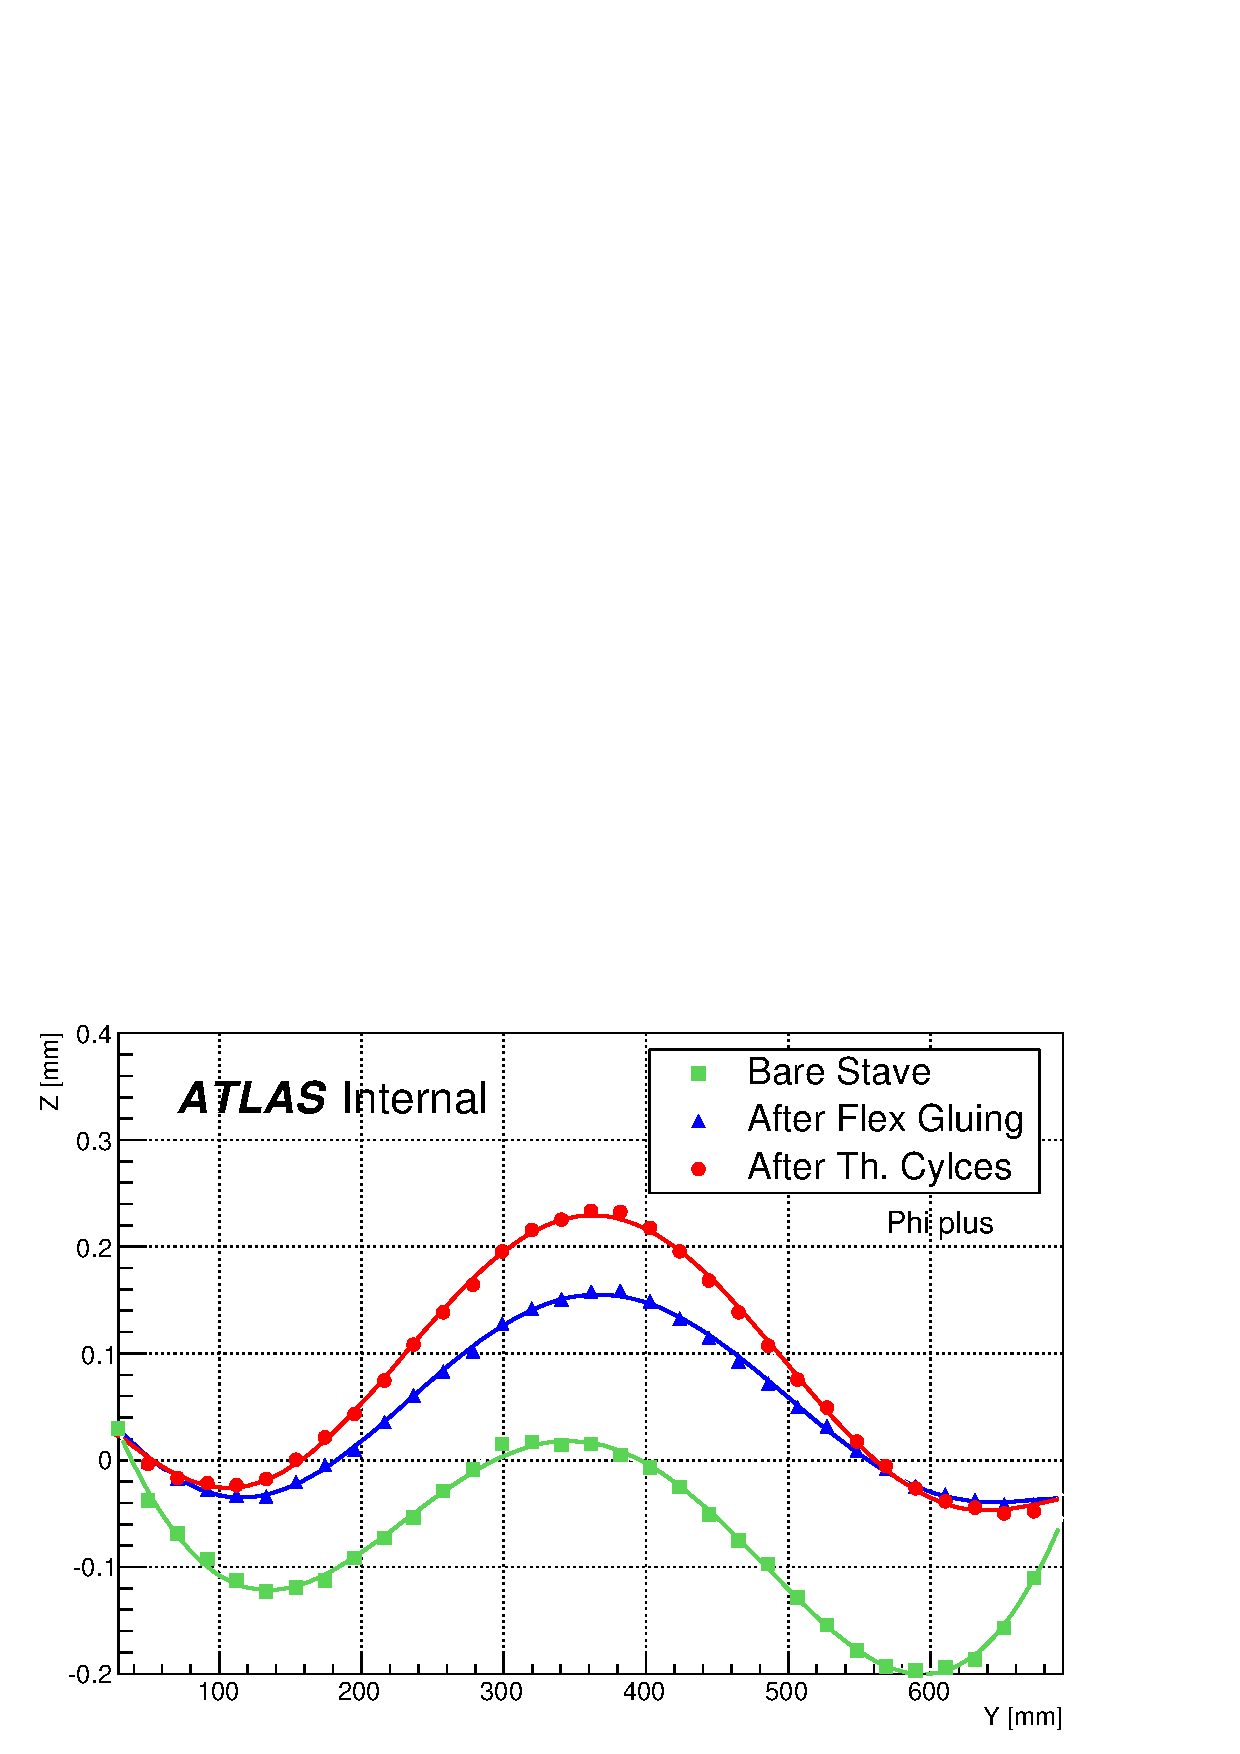
\includegraphics[width=0.35\textwidth]{Images/IBL_Paper/chapter06_LoadingQA/Phi_plus.pdf}}
\caption{Stave profiles before stave flex gluing, after flex gluing and after thermal-cycling at different $\phi$.}
\label{fig:StavePlan_VS_FlexGluing}
\end{figure}

As a first step of the qualification, the staves were visually inspected and the  stave flexes  were  electrically tested to verify that the services were not damaged during the loading. Then  the staves were thermally stressed:  a program was defined with an initial phase at \SI{35}{\celsius} for \SI{1}{\hour} followed by 10 cycles of \SI{1}{\hour} from \SI{40}{\celsius} to \SI{-40}{\celsius}. The program ends with an stabilization phase of \SI{3}{\hour} at \SI{20}{\celsius}~\cite{LoadingNote}.

A metrology survey was systematically done before and after thermal cycling to study how the mechanical supports were deformed by the flex glued on top of them and to verify that the assembly was still respecting the required envelope. The most important measurement of the metrology check was the Planar ity, defined as the maximal excursion from the ideal plane of the stave faceplate surface. The Planar ity of the stave was of importance because of the mechanical envelope of the IBL structure, which allows a clearness of \SI{500}{\micro\meter} during the integration steps of the IBL stave around the IPT. A safe limit for the Planar ity of \SI{350}{\micro\meter} was imposed as a selection cut. The Planar ity results of production staves (before and after thermal cycling) were summarized in Table \ref{table:planarity}~\cite{LoadingNote}. 
The profile of the stave was measured across the cooling pipe direction, three set of measurement were taken, at the center of the stave ($\phi_0$) and at both the edges ($\phi_+$ and $\phi_-$, where the latter refers to the side where the stave flex was glued). An example of one of the stave profile was shown in Figure~\ref{fig:StavePlan_VS_FlexGluing}, showing the measurements for each loading step. The shape of the mechanical supports was changed by the flexes assembly, however they were all still in the envelope.\\
During the prototyping phase one stave flex started to delaminate after several thermal cycles. A carbon clip was added to the design in order to prevent this problem. Out of 22 production assemblies done for IBL, only one stave had a critical problem due to glue mixture mistake and polymerization failure. The remaining assembled staves had gone through a QA procedure to fully qualify the assembly before loading modules onto them. A summary of allocation for the staves was reported in Table~\ref{tab:BareStavesAllocation}.


\begin{table}
\centering
\begin{tabular}{l c  }
\hline \hline
        Type & \#      \\
\hline
Staves accepted for flex assembly & 24 \\
Staves used for system test prototypes & 2 \\
  & \\
Staves assembled with flex  & 22 \\
Staves rejected after flex assembly  & 1 \\
Staves qualified for module loading& 21 \\
Staves loaded with modules  & 20 \\
\hline
\end{tabular}   
\caption{Allocation for the produced and qualified bare staves.
\label{tab:BareStavesAllocation}}
\end{table}



%A metrology survey was systematically done before and after thermalcycling. The latter allows evaluating the Planar ity and possible %change linked to the stress that could build up with temperature in the various layers of the stave.\\
%% show plots for stave 1
%% was stave 15 used? or where was the acceptance limit?


%\subsection{Expected Performance}
%The ATLAS ID provides charged particle tracking with high efficiency in the range $|\eta|~$\textless~2.5 and over the full azimuthal range. 
%Given its radial proximity to the collision region, the existing B-layer provides crucial tracking information: the identification of charged tracks and the reconstruction of multiple collision vertices; subsequent precision   measurements of the reconstruction position, resolution, efficiency and track association for both primary and secondary vertices, and measurements of the b-tagging efficiency as a function of light quark jet rejection. In particular, any inefficiency of the B-Layer results in a severe degradation of the ATLAS physics performance. 
%The addition of the IBL at even smaller radius  will help to preserve the tracking performance and robustness at high luminosity when the B-layer starts to deteriorate from radiation damage, high pile-up occupancy, or the irreparable failure of individual FE-I4 chips or full modules. In addition, given the reduced radial distance to the interaction point and the smaller longitudinal pixel size, the IBL significantly improves the measurement of track transverse ($d_0$) and longitudinal ($z_0 \times$sin$\theta$) impact  parameter resolution.
%A complete evaluation of the expected tracking and vertex reconstruction performance was performed for the IBL Technical Design Report~\cite{Capeans:1291633}. In the meantime the simulation, digitization and cluster reconstruction algorithms had been significantly refined in the view of the start of the Run~2 data taking. A few key performance results in the domain of track reconstruction and $b$-tagging were presented in the following two sections.
%\clearpage

\subsection{Stave Loading}
A description of the stave loading follows. The stave loading was a procedure which consisted of the mechanical loading of the module on the stave and of electrical, functional and mechanical checks of all the stave assembly components.
Reception tests were carried out for the modules and the staves, as soon as they were received from the productions sites, then the modules were loaded onto the staves by mean of dedicated gigs and handling frames. After the module loading the electrical connection from the module to the stave flex were performed with wire-bonds. After this operation, an electrical check of the modules were performed, then the stave was thermally cycled and the electrical checks repeated.
This procedure, as it will be explained in the following subsections, was followed up to the stave number 12, then the last two steps were removed. A module replacement procedure was also available in case of failures of modules.
A detailed description of each part of the stave loading activity follows.


%******************************************
\subsubsection{Module reception tests}
\label{sec:ModuleReceptionTests}
%******************************************
%Module reception test was the procedure devoted to check the functionality of the modules after the shipment from the module production sites to the loading site.
%The module reception tests were devoted to ensure the functionality of the IBL modules after the shipment from the modules production sites to the loading site.

The module reception test procedure consisted  of two steps: optical inspection and electrical check. %Details of these two steps were given in \refsection~\ref{sec:visualinspection} and \refsection~\ref{sec:electricalqualification} respectively.

%------------------------------------------
%\paragraph{Optical inspection}
%\label{sec:visualinspection}
%------------------------------------------
The optical inspection was a thorough visual examination in which the modules were inspected by means of an optical microscope with a total magnification of up to $500\times$ and a digital camera.
The purpose was to check the modules integrity after the transportation to the loading site, especially wire bonds integrity and cracks in the sensor area.
Particular attention was payed to the wire-bondings: each one was checked to make sure there were no shorts, that may had happened due to a shock, nor any weakened or faulty connection. The visible part of the sensors was also inspected for cracks and any other damage that may affect the operation of the module. 
Systematical pictures were taken during the optical inspection, checking systematically:
\begin{itemize}
	\item the fiducial marks, one on each corner of the sensor, since these were the references used during the metrology survey to know the position of a module with respect to the stave fixation reference;
	\item the HV pads, to make sure the pads were well glued and bondings were good, as a failure at this level could prevent the module to be operated.
\end{itemize}
%The optical inspection had proved to be a fundamental step in the modules Quality Assurance tests since it allows the tracking of any aging process that may arise during the IBL production chain.

%\begin{figure}[htb!]
%	\centering
%	\null\hfill
%	\subfloat[Top left corner.\label{fig:topleft}]{%
%		\includegraphics[width=0.3\textwidth]{Images/ibl_stave_loading/ModuleReceptionTest/F12-15-05_top_left_fiducial}
%	}
%	\hfill
%	\subfloat[Top right corner.\label{fig:topright}]{%
%		\includegraphics[width=0.3\textwidth]{Images/ibl_stave_loading/ModuleReceptionTest/F12-15-05_top_right_fiducial}
%	}
%	\hfill
%	\subfloat[HV ring. \label{fig:hvring}]{%
%		\includegraphics[width=0.3\textwidth]{Images/ibl_stave_loading/ModuleReceptionTest/F12-15-05_HV_ring}
%	}
%	\hfill\null
%
%	\null\hfill
%	\subfloat[Bottom left corner.\label{fig:bottomleft}]{%
%		\includegraphics[width=0.3\textwidth]{Images/ibl_stave_loading/ModuleReceptionTest/F12-15-05_bottom_left_fiducial}
%	}
%	\hfill
%	\subfloat[Bottom right corner.\label{fig:bottomright}]{%
%		\includegraphics[width=0.3\textwidth]{Images/ibl_stave_loading/ModuleReceptionTest/F12-15-05_bottom_right_fiducial}
%	}
%	\hfill
%	\subfloat[Global picture.\label{fig:global}]{%
%		\includegraphics[width=0.3\textwidth]{Images/ibl_stave_loading/ModuleReceptionTest/F12-15-05_global}
%	}
%	\hfill\null
 %       \caption{Example of pictures taken during module optical inspection. These pictures show a FBK 3D module (namely F12-15-05).}
 %       \label{fig:visualinspection}
%\end{figure}
%An example of the optical inspection was given in Figure~\ref{fig:visualinspection}.

A total of 456 modules was received and tested for stave production. The number of the modules loaded on the staves and of the ones used for reworkings was showed in \reffigure~\ref{figure:numodules}.

\begin{figure}
	\centering
	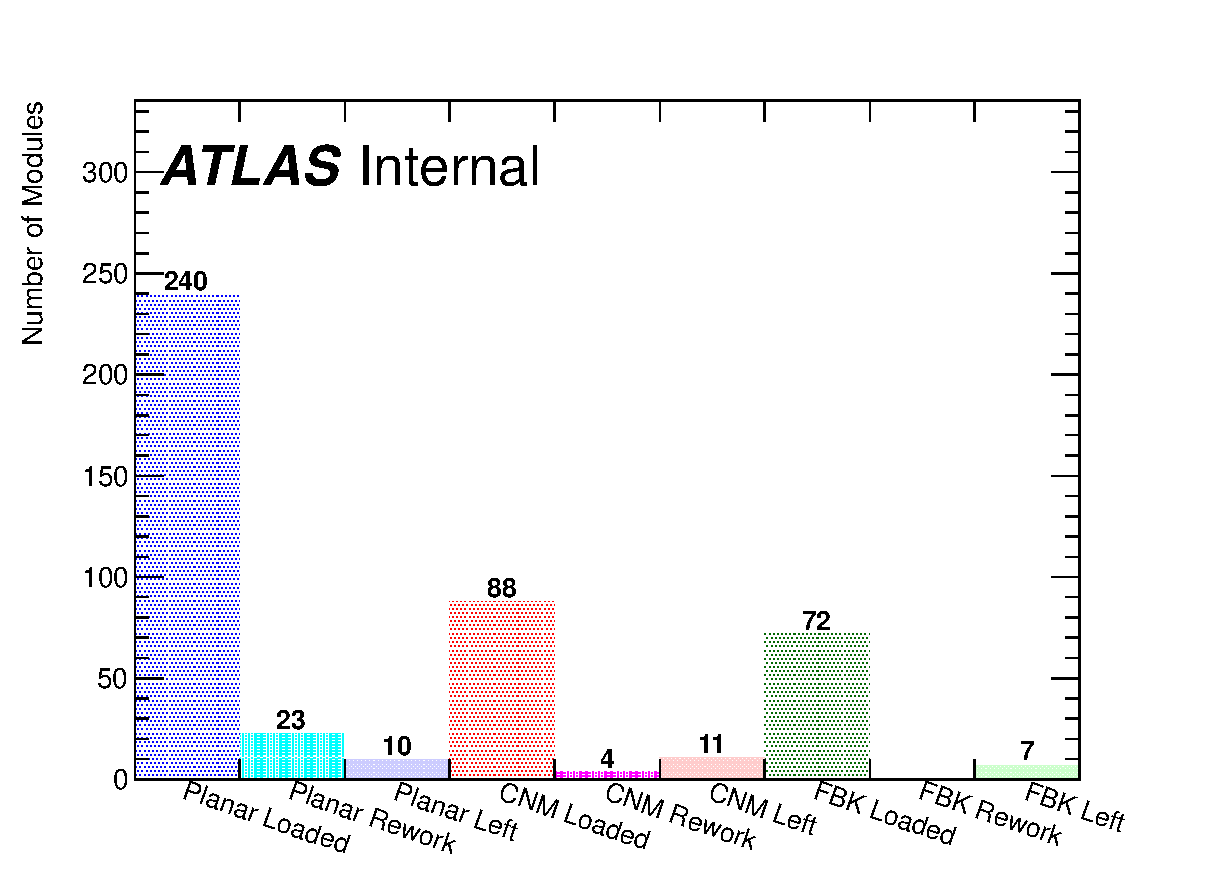
\includegraphics[width=0.6\textwidth]{Images/ibl_stave_loading/ModuleReceptionTest/modules.eps}
	\caption{Total number of modules tested (planar, 3D CNM and 3D FBK) organized in categories.}
	\label{figure:numodules}
\end{figure}


%The results obtained during the reception tests were systematically compared to the module Quality Assurance, QA, results at the production sites.
%At every stages of the reception test procedure, a comparison between the results at the loading site and the informations reported on the module traveller document had been done }.
%For the final ranking of the modules, in addition to the defective pixel, was also taken in consideration if there was an high leakage current or a smaller operational margin. These tests were translated into a number of additional defective pixel. Moreover other criteria were also taken into account, like a rework of the module which can concern the chip, the wire-bond or the module flex. Module with a number of bad pixel less than 270 per FE chip, i.e. 270 for 3D modules and 540 for Planar  modules respectively, were of good quality. Modules showing more than 270 bad pixel were discarded from further integration. In addition modules showing less 100 bad pixel per FE-chip were of best quality.
No module was rejected at the optical inspection stage.
%At the stage of optical inspection, no particular issues were found for the modules with respect to the production sites, confirming that no damage had been caused during the transportation. %\marginpar{should we mention something special here?}\\

The electrical and functional checks of the modules consisted in the repetition of some of the tests already performed during the module quality assurance. In this test the functionality of the readout chip had been retested, checking the performance of both the digital and the analog part of the chip. Threshold scans were as well performed, and a tuning of the chip repeated. Those steps were not meant to qualify the module, but just to check that the FE was not damaged during the transportation and it was still showing the same behavior measured at the production site. Pictures of the setup for electrical tests are shown in Figure~\ref{figure:USBpixsetup}

\begin{figure}
	\centering
	\null\hfill
	\subfloat[\label{fig:setup}]{%
		\includegraphics[width=0.4\textwidth]{Images/ibl_stave_loading/ModuleReceptionTest/setup}
      }
	\null\hfill
	\subfloat[\label{fig:adaptercards}]{%
		\includegraphics[width=0.4\textwidth]{Images/ibl_stave_loading/ModuleReceptionTest/adaptercards}
       }
\hfill\null
       \caption{The USBpix setup used for the electrical qualification of the modules. \reffigurecapital~\ref{fig:setup} shows the USBpix setup for single (left) and double (right) chip modules. \reffigurecapital~\ref{fig:adaptercards} shows the USBpix adapter cards used for the electrical qualification of the modules.}
        \label{figure:USBpixsetup}
\end{figure}


The electrical characteristics of the sensor were checked by mean of an I-V scan, monitoring the voltage breakdown, defined as in the production site and the operational current. 
\reffigure~\ref{figure:breakmodule} shows the distribution of the measured breakdown voltage values, V$_{\mathrm{bd}}$, for the complete IBL modules population received at the loading site. The minimum V$_{\mathrm{bd}}$ observed for the Planar  sensors was 130~V and 95\% of them had values greater than 200~V. For what concerns the 3D sensors, the sensors from the two producers present different performances: the breakdown distribution of the FBK production had a mean value of 42.5~V and a root mean square value of 7~V, while the CNM sensors present a flat distribution between 20~V and 105~V.
%The difference between the two 3D sensors flavours voltage breakdown value was due to the sensor test procedure since the CNM sensor I-V characteristics was performed using the guard ring as ground contact. %From the guard ring it's not possible to deplete the whole sensor getting blind to some bulk effects with a result of a broader distribution with respect to the FBK modules.\\
%The difference between the two 3D sensors flavours voltage breakdown value was due to the sensor test procedure since the CNM sensor I-V characteristics was performed using the guard ring as ground contact. In this way the value of the current was dominated by the surface one making the measurement of the breakdown difficult with the result of a broader distribution with respect to the FBK modules.  
The measurement of the I-V curve only on the guard ring used by CNM at wafer level did not allow to properly extrapolate the breakdown voltage value at the tile level as was done in the FBK case, where the measurement was performed on the full device, leading to a broader distribution. Fourteen CNM sensors presented a linear (ohmic) increase of current as a function of the increasing bias voltage in the explored range: in these cases the breakdown was most probably larger than the maximum voltage (100~V). No significant discrepancies had been found with respect to the production sites in terms of operational currents and breakdown voltages. In the very few cases where a lower V$_{\mathrm{bd}}$ value was observed, the modules had been rejected.
%with respect to the production site, modules had been discarded from being a candidate for the stave loading.
%\marginpar{should we add how many modules presented such behavior?}\\% additional penalties had been given in order not to use the module as first choice although still would fell in the IBL specifics. \\
%For what concern the functional tests, no significant differences had been found considering the bad pixels analysis (which takes into account the digital, the analog and the threshold scans) with respect to the analysis made in the production site, confirming any loss in the quality of the modules. \\
%Less then 10 modules had been rejected due to communication issues with the FE-I4 electronics. Whenever a problem in communication between the USBPix read-out system and the module occurred, a further check with the Reconfigurable Cluster Element (RCE) read-out system was performed. If the communication problem was confirmed, the module was disqualified.

The modules loaded on the staves were selected according to the ranking of the modules assigned at the production site and the V$_{\mathrm{bd}}$.

For the reception test analysis purpose and for a quick check of the stave functionality, an analysis framework had been developed at the loading site. The software, which includes the ROOT libraries, was largely used for example to compare the results at each stages of the staves production (before/after loading, before/after thermal cycle, etc..), to find failing pixels or just to investigate problems in a faster way. 

\begin{figure}
      	\centering
	\null\hfill
	\subfloat[Typical I-V behavior for Planar  and 3D sensors. A current limit of -20~\microA\ was used to protect the modules.\label{figure:ivmodules}]{%
		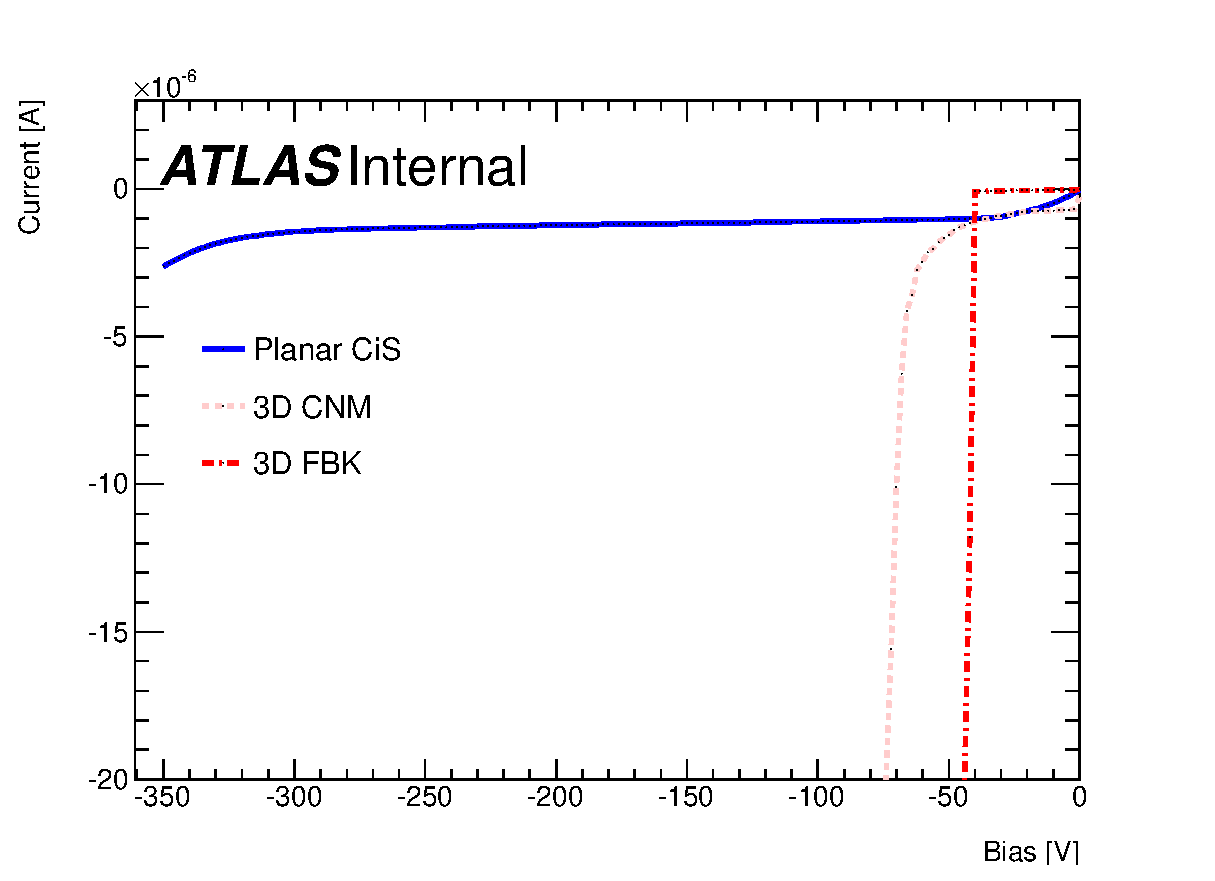
\includegraphics[width=0.49\textwidth]{Images/ibl_stave_loading/ModuleReceptionTest/iv_alltec.eps}
	}
	\hfill
	\subfloat[Breakdown values measured for all the modules.\label{figure:breakmodule}]{%
		\includegraphics[width=0.49\textwidth]{Images/ibl_stave_loading/ModuleReceptionTest/Vbd_distribution.eps}
	}
	\hfill\null
        \caption{Typical I-V curves of the modules and the measured breakdown values distribution.}
        \label{figure:IVDistro}
\end{figure}

%\begin{figure}[htb]
%\centering
%\includegraphics[width=0.7\textwidth]{Images/ibl_stave_loading/ModuleReceptionTest/Vbd_distribution.eps}
%\caption{Breakdown values measured for all the modules.}
%\label{figure:breakmodule}
%\end{figure}
%*****************************************

%------------------------------------------
\subsubsection{Module loading procedure}
\label{subsec:LoadProc}
%------------------------------------------
The first step in the loading procedure was the selection of the 12 Planar  and the 8 3D sensor modules to be loaded on one stave out of the ones available in stock at that moment. 
Due to the HV modularity, modules with similar breakdown performance were chosen for the same HV sector. Moreover FBK and CNM 3D modules were not mixed in the same HV group. The strategy adopted was to choose the modules with best ranking available for the more central positions, both for Planar  and 3D modules.
%After the module selection, the loading was characterized of several delicate mechanical steps, ensuring mechanical strength, precise positioning, minimization of dead regions area and material budget.
%Due to the mechanical design, minimizing the material budget and dead regions, the loading procedure was performed in several delicate steps ensuring a proper mechanical strength and a precise positioning.

At first the stave was positioned and aligned on the loading tool (\reffigure~\ref{figure:staveloadingprep}), which provided support and the reference points for the loading procedure, protecting the stave.
The reference points were used for a precise positioning of the stave in the tool itself.
\begin{figure}[h!]
\centering
        \includegraphics[width=0.8\textwidth]{Images/ibl_stave_loading/MainLoading/1.jpg}
        \caption{3D model of a stave and its handling frame positioned on the loading tool.}
       % On the stave side, we can observe in green the intermediate PCB loaded on the handling frame extenders and the stave-flex in orange. On the loading tool side, the staves-flex wings protector was represented in blue and the rails used for the optical inspection in orange.}
        \label{figure:staveloadingprep}
\end{figure}

Once the stave alignment was performed, a 70~\microm\ thick stainless steel mask was positioned on the stave \faceplate\
%Once the stave alignment was performed, the module loading jig was moved in place for the loading of the first module, allowing the positioning of a 70~\microm\ thick stainless steel mask
%Once the stave alignment was performed, the module loading jig was moved to a dedicated work bench and the first loading step can start with the positioning of a 70~\microm\ thick stainless steel mask
 (\reffigure~\ref{fig:maskpositioning})\footnote{Due to the tool design, the loading was done one side at a time, without any preference between A or C side. This side-to-side sequential loading was mainly due to the needed alignment tools in the central region that will overlap in the case of a parallel loading (see \reffigure~\ref{fig:positioningstopers} for an example).}, which allowed the deposition of a $\sim$70~\microm\ thick layer of thermal grease\footnote{\href{http://www.electrolube.com/products/thermal-management/91/16/}{HTCP}, Electrolube.}, ensuring good thermal contact between the \faceplate\ and the module (\reffigure~\ref{fig:thermalgreaseapli}). In order to obtain sharp edges, the stainless steel shim was previously sprayed with a universal adhesive for large surface bonding produced by UHU and temporarily glued to the \faceplate. %while applying the thermal grease.
%When the mask was removed a clean pattern of thermal grease was revealed as shown in \reffigure~\ref{fig:greaseandglue}.
The use of a mask allowed two points per FE-I4 to be left clean in order to apply glue drops which will bond the modules to the \faceplate (Figure \ref{fig:greaseandglue}).
%The mask allowed to leave some empty spots in the thermal grease shape. It allows hosting the glue dots, which will bond the modules on the stave \faceplate.
 
A positioning jig with plastic stoppers was then installed to constrain the module to be loaded on the $x$-axis all along the stave and on the $y$-axis for the central module, as shown in \reffigure~\ref{fig:positioningstopers}. Two Araldite 2011\footnote{\href{http://www.meury.com.au/ProductDisplay.asp?PID=48}{Araldite 2011}, Meury Enterprises TY LTD.} glue drops per FE-I4 chip were then applied with a needle on the thermal grease template openings. The first module was then loaded and pushed against the stoppers while a 205~\microm\ thick spacer was placed as shown in \reffigure~\ref{fig:spacerandon} with a holder block. This spacer setted the module-to-module distance, allowing a later insertion of an electric insulator, but also preventing any tilt angle of the module. The same procedure was then repeated for all the modules in the same half of the stave. An extra positioning tool, equipped  with plastic stoppers, was used at this point, Fig.\,\ref{fig:positionover}.

Weights of 20~g were positioned on top of the modules, one for each FE-I4 readout chip, during the glue curing process (24 hours at room temperature), helping the module to properly settle on the grease layer and the glue dots contacts (\reffigure~\ref{fig:loadingweights}). In order to prevent any damage to the module the weight was equipped with three Teflon feets in order to leave space for the wire-bonds and the loaded SMDs. The weight and positioning tools were then removed (\reffigure~\ref{fig:loadingdismount}) and an optical inspection was performed for each FE-I4 electronic chip thanks to a built-in sliding camera (\reffigure~\ref{Fig:loadingopticalInspec}).

The full process was then repeated on the other side of the stave.

\begin{figure}
	\centering
	\null\hfill
	\subfloat[Positioning of the aluminum mask (in green) and thermal grease application.\label{fig:thermalgreaseapli}]{%
		\includegraphics[width=0.3\textwidth]{Images/ibl_stave_loading/MainLoading/3.jpg}
	}
	\hfill
		\subfloat[Installation of the last positioning stopper.\label{fig:positionover}]{%
		\includegraphics[width=0.3\textwidth]{Images/ibl_stave_loading/MainLoading/7.jpg}
	}
	\hfill
	\subfloat[Installation of the module weights.\label{fig:loadingweights}]{%
		\includegraphics[width=0.3\textwidth]{Images/ibl_stave_loading/MainLoading/8.jpg}
	}
	\hfill\null
        \caption{3D representations of each of the main stave module loading steps.}
        \label{fig:moduleloading}
\end{figure}

%------------------------------------------
%\paragraph{\upcase \staveflex\ wing gluing and wire-bonding}
\label{subsec:WingGluingWireBonding}
%------------------------------------------
%Once a stave was fully loaded or a module replaced\footnote{For simplicity the following wing gluing description will be in plural as for a non reworked stave, being the only difference that for a reworked stave only the affected module wings need to be glued.}, we proceed with the stave wing gluing.
%Each FE having its own independent wing providing power and signals they need to be glued independently.
After the glueing of the modules to the support stave, the stave flex was glued to the module flex.
%Once all the modules were glued on the stave, the electrical connection between the \staveflex\ services and the modules can start. This consisted  of several steps which were listed below.
A layer of Araldite 2011 was deposited in correspondence of the \staveflex\ wings (\reffigure~\ref{fig:gluestamp} and \reffigure~\ref{fig:gluedepo}) through a mask (\reffigure~\ref{fig:maskwing}), in order to apply the glue only in the desired area.
The wings were then released and positioned on the module flex (\reffigure~\ref{fig:winghandpos}) before installing the wing positioning tool. This tool locked the stave in its position by means of a wedge which pushed against the stave, allowing the wings to stay in their nominal position by using two clamps. All the wings were retracted and bent away to leave access to spray the glue. A weight of 16~g was then positioned on top of the wing during the glue curing process. In order to avoid any glue excess or damage to the module nor to the wing pads, the weight contact surface was covered with Teflon.

Once the stave was fully loaded and cured, a Kapton insulator of $\sim$100~\microm\ was inserted in between each powering sector for HV electrical insulation purposes (\reffigure~\ref{fig:hvinsu}). The insulator was constrained to an holder (Fig. \reffigure~\ref{fig:hvinsu}) glued to the module flexes, avoiding any leak of glue in the space between the module. This operation prevented to had shorts in between the modules.
In order to avoid any glue between the modules, a holder was glued to two consecutive \moduleflex es which holds the insulator. As a last step, the stave envelope was checked to fulfil the mechanical constrains of the IBL, as shown on \reffigure~\ref{fig:envcheck}

\begin{figure}
	\centering
	\subfloat[Wing positioning for each FE.\label{fig:winghandpos}]{%
		\includegraphics[width=0.3\textwidth]{Images/ibl_stave_loading/WingGluing/5.jpg}
	}\quad
	\subfloat[HV insulator placement and bridge gluing.\label{fig:hvinsu}]{%
		\includegraphics[width=0.3\textwidth]{Images/ibl_stave_loading/WingGluing/10.jpg}
	}\quad
	\subfloat[Stave envelope check.\label{fig:envcheck}]{%
		\includegraphics[width=0.3\textwidth]{Images/ibl_stave_loading/WingGluing/IBL_STAVE_ENVELOPE_JIG_ISO-01.jpg}
	}
	\caption{3D representations for each of the main stave-flex wing gluing steps.}
	\label{fig:winggluing}
\end{figure}

Modules HV, clock, command, data output lines and powering pads were wire-bonded to the respective wing pads with 25~\microm\ AlSi (1\%) wires. For redundancy, four wire-bonds were performed per Low Voltage Differential Signaling (LVDS) and HV pad. Ten wire-bonds were dedicated to the LV and the ground to cope with the expected 0.5~A current per FE. 
For the wire-bonding operation, the stave and its handling frame were installed into the wire-bonding cradle. To ensure a good support and stiffness of the wire-bonded region, a shim block was positioned underneath the stave stave). The bond-loop height was limited to a maximum value of 250~\microm. Wire-bonds quality was tested by pull tests, performed every 2 FE on empty pads. The results of the pull tests were reported in \reftable~\ref{table:wire-bond}.
\begin{table}
	\centering
	\begin{tabular}{|l|c|c|c|c|c|}
  		\cline{2-6}
		\multicolumn{1}{r|}{} & stave 1 & stave 2 & stave 3 & stave 4 & stave 5 \\
  		\hline
		Mean pull force [g$_{\mathrm F}$] & $6.23 \, \pm \, 0.78 $ & $5.70 \, \pm \, 0.59 $ & $6.13 \, \pm \, 0.63 $ & $5.75 \, \pm \, 0.62 $ & $5.94 \, \pm \, 0.43 $ \\
		\hline
		\noalign{\smallskip}
  		\cline{2-6}
		\multicolumn{1}{r|}{}  & stave 6 & stave 7 & stave 8 & stave 9 & stave 10 \\
  		\hline
		Mean pull force [g$_{\mathrm F}$] & $6.22 \, \pm \, 0.74 $ & $6.30 \, \pm \, 0.64$ & $6.23 \, \pm \, 0.51 $ & $5.85 \, \pm \, 0.53 $ & $6.09 \, \pm \, 0.58$ \\
		\hline
		\noalign{\smallskip}

  		\cline{2-6}
		\multicolumn{1}{r|}{}  & stave 11 & stave 12 & stave 13 & stave 14 & stave 15 \\
  		\hline
		Mean pull force [g$_{\mathrm F}$] & $6.19 \, \pm \, 0.56$ & $6.00 \, \pm \, 0.69$ & $7.20 \, \pm \, 0.29$ & $7.26 \, \pm \, 0.33$ & $6.80 \, \pm \, 0.50$ \\
		\hline
		\noalign{\smallskip}

  		\cline{2-6}
		\multicolumn{1}{r|}{}  & stave16 & stave 17 & stave 18 & stave 19 & stave 20 \\
  		\hline
		Mean pull force [g$_{\mathrm F}$] & - & $7.11 \, \pm \, 0.41$ & $7.03 \, \pm \, 0.42$ & $ 6.32 \, \pm \, 0.66 $ & $5.85 \, \pm \, 0.76$ \\
		\hline
		\noalign{\smallskip}
	\end{tabular}
	\caption[Table caption text]{Mean and RMS values of the wire-bonds pull tests performed on the 20 staves produced. Values for stave 16 were lost.}
	\label{table:wire-bond}
\end{table}

%Half-way through the stave production, degradation of the wire-bond quality was observed due to corrosion phenomena. 
%The activation of this corrosion was identified to be correlated to the humidity level during the thermal cycle procedure. Stave temperature and humidity were monitored during a thermal cycle (\reffigure~\ref{fig:dewpoint_thermal}) showing that the dew point was reached during the fast temperature ramp-up due to the large volume of the climate chamber (1.6~m$^3$).  Thermal cycle on loaded staves was thus given up starting from stave 13. For the first twelve staves assembled, a dedicate re-bonding procedure was performed at the CERN Detector Silicon Facility (DSF) laboratory to recover all affected modules. All module flex to stave flex wire-bonds had been systematically redone after a proper pad cleaning. Front-end to module flex wire-bonds were redone case by case after a careful evaluation, due to the mechanical fragility of the FE-I4 pads leaning out of the stave. The integrity (mechanical structure and electrical integrity) of thermal cycled staves was confirmed by metrology measurements and electrical characterizations.

\begin{figure}
	\centering
        \includegraphics[width=0.6\textwidth]{Images/ibl_stave_loading/WingGluing/IMG_3091.JPG}
        \caption{\upcase \staveflex\ wings under wire-bonding showing the wire-bonding head and the shims placed under the stave to increase its mechanical stability.}
        \label{fig:shimforwire-bonding}
\end{figure}

%\begin{figure}[h!]
%	\centering
%        \includegraphics[width=0.8\textwidth]{Images/ibl_stave_loading/ThermalCycle/StaveThermalcyleDewPoint.eps}
%        \caption{Figure showing the stave temperature and humidity during the thermal cycle. The computed dew point (stars line) was exceeded during the temperature ramp up by the stave temperature (doted line).}
%        \label{fig:dewpoint_thermal}
%!TEX encoding = UTF-8 Unicode\end{figure}


%------------------------------------------
\paragraph{Module replacement procedure}
\label{subsec:ModReplacement}
%------------------------------------------
A module replacement procedure was developed, during the stave production period, in order to replace any failing module that was already loaded on a stave. Figure~\ref{fig:ReworkModules} shows how many modules were reworked and for which reason.
%A re-working module procedure had been developed for replacing any failing module loaded on a stave.
In total, fifteen reworks were performed due to modules being accidentally damaged during the module loading procedure, thus compromising the integrity of the sensor, the FE-I4 or the \moduleflex; five modules had been replaced due to failures of the FE-I4 chip and two more modules had been replaced because they had failed the QA tests performed before final integration.
%Due to the wire-bonding corrosion observed on the first twelve staves assembled, a dedicate re-bonding procedure was performed at the CERN Detector Silicon Facility (DSF) laboratory to recover all affected modules. All \moduleflex\ to \staveflex\ wire-bonds had been systematically redone after a proper pad cleaning. Front-end to \moduleflex\ wire-bonds were redone case by case after a careful evaluation, due to the mechanical fragility of the FE-I4 pads leaning out of the stave.
In addition, due to the cleaning and re-bonding intervention performed at DSF, six more module were replaced on the twelve re-bonded staves.
The statistics of the module replacements were shown in \reffigure~\ref{fig:ReworkModules}.
%This need was mainly driven by the mechanical damaging of modules during the loading, representing 68\% of the re-worked module as can be seen in \reffigure~\ref{fig:ReworkModules}. Although loaded modules had been qualified and tested before their loading, some disfunctionalities can show after the loading due to the applied mechanical stress\footnote{Mechanical stress on the modules can affect to their break down voltage or indirectly to some FE functionalities.} or infant-mortality ($23\%$ re-works).

\begin{figure}
	\centering
        \includegraphics[width=0.7\textwidth]{Images/ibl_stave_loading/MainRework/reworked_modules.eps}
        \caption{Number of modules for each category of rework. Reworks were mainly motivated by accidents during the loading or modules re-bonds and FE failures during the early testing. A minority were replaced after the stave QA due to some failing registers.}
        \label{fig:ReworkModules}
\end{figure}

The module replacement procedure\footnote{In order to avoid any repetition, only the instructions that differ from to the standard module loading procedure were mentioned in this section.} started with the installation of two 100~\microm\ thick Kapton spacers between the module that needed to be removed and its neighbors. Spacers of only 100~\microm\ were placed during the module rework instead of 205~\microm\ in order to add some margin to the module placement.
The spacers maintained the distances between the modules and protect the neighboring modules. The failing module was then removed by inserting a plastic spatula in between the module and the \faceplate, breaking the glue drop bonds. The \faceplate\ was then cleaned to remove any thermal grease and glue. A new thermal grease layer was then applied by using an individual mask. Once the mask was removed, glue drops were applied and the new module was placed thanks to a dedicate individual positioning tool. A weight of 20~g for the 3D modules or 40~g for the Planar  modules was then put on top during the glue curing process.

After the module placement, the wing gluing, the optical inspection, the envelope check and the HV insulator insertion were performed following the same procedure as for the standard loading.

%\begin{figure}
%        \centering
%        	\null\hfill
%	\subfloat[Installation of the module spacer and neighbors protection.\label{fig:replacementprotection}]{%
%		\includegraphics[width=0.3\textwidth]{Images/ibl_stave_loading/MainRework/1.jpg}
%	}
%	\hfill
%	\subfloat[Module ungluing and \faceplate\ cleaning.\label{fig:moduleoutandcleaning}]{%
%		\includegraphics[width=0.3\textwidth]{Images/ibl_stave_loading/MainRework/2.jpg}
%	}
%	\hfill
%	\subfloat[Thermal grease mask installation.\label{fig:indmaskgrease}]{%
%		\includegraphics[width=0.3\textwidth]{Images/ibl_stave_loading/MainRework/3.jpg}
%	}
%	\hfill\null
%
%	\null\hfill
%	\subfloat[Thermal grease pattern and glue dots.\label{fig:gluedropsrework}]{%
%		\includegraphics[width=0.3\textwidth]{Images/ibl_stave_loading/MainRework/4.jpg}
%	}
%	\hfill
%	\subfloat[Module placement thanks to the positioning tools.\label{fig:modulpostrework}]{%
%		\includegraphics[width=0.3\textwidth]{Images/ibl_stave_loading/MainRework/5.jpg}
%	}
%	\hfill
%	\subfloat[Weight positioning and glue curing.\label{fig:weightrework}]{%
%		\includegraphics[width=0.3\textwidth]{Images/ibl_stave_loading/MainRework/6.jpg}
%	}
%	\hfill\null        
%	\caption{3D representations of each of the main module replacement steps.}
%\end{figure}

\subsubsection{Stave quality check at the loading site}

%******************************************
%\section{Stave quality check}
\label{sec:Stave_QC}
%******************************************

%------------------------------------------
%\paragraph{Metrology survey}
%------------------------------------------
A stave quality check was performed for each stave, aiming to spot possible damages occurred to the instrumented stave after the loading procedure and to perform aging tests.
The stave quality check consisted of a metrical check of module position and electrical and functional tests of the loaded modules. A thermal cycle of the stave after the loading was as well part of the procedure, but this operation was stopped after having built the first 12 staves due to an observed condensation phenomena. This issue was threaten in details in the stave quality assurance section of this chapter.
Both the metrical, electrical and functional tests were performed before and after the thermal cycle procedure.\\
The position of the modules was checked by means of a metrology machine.  A pattern recognition of the sensors was performed and the $x$, $y$ and $z$ coordinates were obtained by probing the fiducial marks.%, as shown in \reffigure~ \ref{fig:probinghead}. 
%The position along the $z$-axis was obtained by probing each module at each corner, as shown in \reffigure~ \ref{fig:probinghead}. 
%Modules position was checked after loading thanks to the metrology machine. The handling frame and stave were positioned on the granite table in a defined position while the stave cover was removed. The position in $z$ was obtained by probing the module at 4 different locations, as shown on \reffigure~\,\ref{fig:probinghead}.
In order to fit in the IBL volume a stave needed to had a maximal excursion of \SI{0.35}{\milli\meter}, this was also checked as described in the loading procedure in the envelope check, that was repeated also after the thermal cycle. The profile of each stave was as well measured during the metrical test, in order to had a complete monitoring. The results on the staves $z$-axis profiles were shown in \reffigure~ \ref{fig:staveprof} for the test performed before the thermal cycle procedure, divided between $\phi^+$ and $\phi^-$.
%Results were shown in \reffigure~ \ref{fig:staveprof}, \marginpar{what was $\phi^\pm$?} where the stave $z$ profile was shown for $\phi^+$ and $\phi^-$.

%\begin{figure}
%        \centering
%	\includegraphics[width=0.49\textwidth]{Images/ibl_stave_loading/Metrology/IMG_3677.JPG}
%	\caption{Stave metrology after loading. Picture showing the probing of a 3D module.}
%	\label{fig:probinghead}
%\end{figure}

The position of each module, measured during the process, was compared to the nominal design position.
%\reffigurecapital~ \ref{fig:loadingpre} shows the distributions of the modules residuals with respect to the nominal $(x, y)$ positions. 
The RMS of the residual distribution was of $\sim$50~\microm\ for Planar  modules in both axes and $\sim$34~\microm\ in $x$ and $\sim$57~\microm\ in $y$ for 3D modules.

%Error distributions of the module loading position in the $xy$ plane was shown in \reffigure~\,\ref{fig:loadingpre} for the $x$ and $y$ axis showing a module loading positioning precision of $50 \, \mu m$ for Planar  in both axes and $56 \,  \mu m$ in $x$ and $33 \, \mu m$ in $y$ for 3D.
%Mean value for the $x$ axis was 50 with a RMSD of $TBC$ and the mean value for the $y$ axis was $TBC$ with a RMSD of $TBC$.

\begin{figure}
	\centering
	\subfloat[Loaded staves Planar ity ($\phi^-$).\label{fig:staveplanarityphiplus}]{%
		\includegraphics[width=0.5\textwidth]{Images/ibl_stave_loading/Metrology/PlanarityUniGeMinus.eps}
	}
	\subfloat[Loaded staves Planar ity ($\phi^+$).\label{fig:staveplanarityphiminus}]{%
		\includegraphics[width=0.5\textwidth]{Images/ibl_stave_loading/Metrology/PlanarityUniGePlus.eps}
	}
	\caption{Average profiles of the 20 staves produced (black dots) along the $z$-axis and divided between $\phi^+$ and $\phi^-$. The filled boxes represent the range of values measured for the profiles.}
	%Maximum and minimum measured $z$ values at each measurement point were represented by the filled area.
	\label{fig:staveprof}
\end{figure}

%\begin{figure}
 %       \centering
 %       \null\hfill
  %      \subfloat[Planar modules $x$ residuals.\label{fig:planarpositionx}]{%
%		\includegraphics[width=0.4\textwidth]{Images/ibl_stave_loading/StaveTest/PositioningX_planar.pdf}
%	}
  %      \hfill
     %   \subfloat[Planar modules $y$ residuals.\label{fig:planarpositiony}]{%
%		\includegraphics[width=0.4\textwidth]{Images/ibl_stave_loading/StaveTest/PositioningY_planar.pdf}
%	}
   %     \hfill\null
      %  
       % \null\hfill
%        \subfloat[3D modules $x$ residuals\label{fig:3Dpositionx}]{%
%		\includegraphics[width=0.4\textwidth]{Images/ibl_stave_loading/StaveTest/PositioningX_3D.pdf}
%	}
%        \hfill
%        \subfloat[3D modules $y$ residuals\label{fig:3Dpositiony}]{%
%		\includegraphics[width=0.4\textwidth]{Images/ibl_stave_loading/StaveTest/PositioningY_3D.pdf}
%	}
%	\hfill\null
%	\caption{Residual values of the modules fiducial marks with respect to their nominal position in $x$ and $y$ directions for both sensor technologies.}
%	\label{fig:loadingpre}
%\end{figure}

%------------------------------------------
%\paragraph{Electrical and functionality quality check}
\label{subsec:ElecFuncQC}
%------------------------------------------
The aim of the electrical check was to spot any possible damage that may had occurred during one of the assembly, wire-bonding or metrology survey steps. A full electrical qualification of the module followed after the stave being delivered at the integration site.
%The standard procedure consisted  in two tests, each of them performed after the two metrology surveys foreseen by the loading procedure.
%For the reworked staves, additional tests had been performed in order to monitor the staves behavior after each intervention.

%The electrical quality check procedure consisted  of the same tests performed during the module reception-tests\footnote{the deatails of each scan can be found in Appendix A} and a dedicated tuning procedure.
\begin{figure}
	\centering
	%\hfill
	%\subfloat[Modules threshold distributions.\label{fig:_StaveRes.b}]{%
	%	\includegraphics[width=0.45\columnwidth]{Images/ibl_stave_loading/StaveTest/OvThresholdDistro.eps}
	%}
	\hfill
	\subfloat[Modules ENC distributions.\label{fig:_StaveRes.b}]{%
		\includegraphics[width=0.45\columnwidth]{Images/ibl_stave_loading/StaveTest/OvNoiseDistro.eps}
	}
	\hfill
	\subfloat[Modules breakdown distribution.\label{fig:_StaveRes.a}]{%
		\includegraphics[width=0.45\columnwidth]{Images/ibl_stave_loading/StaveTest/StaveBKDdistro.eps}
	}
	\caption{Stave quality results:  (a)Equivalent Noise Charge, ENC, of the modules loaded on the staves for each pixel technology and producer; voltage breakdown (b) for each HV sector of the production staves, the last bin was the overflow bin, for breakdown values higher than 350~V.}
	\label{fig:_StaveRes}
\end{figure}
%\clearpage

%------------------------------------------
%\subsubsection{Setup}
%------------------------------------------
The stave testing setup is schematized in \reffigure~\ref{fig:_StaveSetup} and a photo is presented in \reffigure~\ref{fig:_StaveSetupPic}.

\begin{figure}
	\centering
	\null\hfill
	\subfloat[\label{fig:_StaveSetup}]{\includegraphics[width=0.8\textwidth]{Images/ibl_stave_loading/StaveTest/StaveSetup.png}}
	\hfill\null
	\null\hfill
	\subfloat[\label{fig:_StaveSetupPic}]{\includegraphics[width=0.8\textwidth]{Images/ibl_stave_loading/StaveTest/StaveSetupPic.jpg}}
	\caption{(a) Sketch of the stave testing setup, (b) Picture of the stave testing setup.}
\end{figure}
During those tests the staves were powered and cooled for the first time, the stave temperature was set to \SI{19}{\celsius}. For the stave cooling, a two phase CO$_2$\cite{traci} system was used, in order to not contaminate the cooling pipes with other coolant liquids. The system was able to cool the staves between \SI{-35}{\celsius} and \SI{20}{\celsius}, providing a maximum cooling power of about \SI{250}{\watt}.
%this was reported by nikhef
%The experimental setup for the stave quality check needs to be close to the official ATLAS one. Since CO$_2$ will be used during data-taking as cooling system, in order to avoid any kind of contamination of the cooling pipes, the same system with lower power capacity was used for the stave quality check:
%\cite{TRACI}
A custom Detector Control System (DCS) was developed for the monitoring of temperature and humidity of the stave environment. This DCS was based on a National Instrument board\cite{NIboard}, instrumented with humidity and temperature sensors, and LabView software. An interlock had been set to prevent modules to reach temperatures above \SI{40}{\celsius}.
The DCS system was capable as well of monitoring the module temperatures thanks to the NTC located on the module flex.
%whenever a module temperature was exceeding $40^{\circ}$C, so that, in such case a power cut of the stave was performed. %the stave powering system had got a power cut.\\
%The powering of the stave requires Low Voltage (LV) and High Voltage (HV) supplies: the first ones were meant for the FE readout chips while the second ones were for the depletion of the silicon sensors.
%Four LV power supplies had been used to take care of the powering of the FEs. Each power supply had two powering channels, thus making possible the simultaneous operation of the eight LV channels needed for a stave. 
An external Low Voltage regulator system was developed to ensure that the LV regulation does not accidentally exceed the limit of \SI{2.4}{\volt}, in order to not damage the LDOs on the readout chip. An ISEG\footnote{\href{http://www.iseg-hv.com/products/crates/}{iseg system crates}, iseg Spezialelektronik GmbH.} crate was used for the HV power of the silicon sensors. This HV power supply was able to reach up to 1000~V, while the scans were limited to \SI{350}{\volt}. A dedicated Labview program was developed for monitoring and for interlock purposes. The software interrupted the power on a channel if the current got higher than \SI{100}{\micro\ampere}.

The DAQ setup was made of two RCEs and two High Speed Input/Output (HSIO)\cite{RCE} boards which communicate through optical fibers.
%In particular, the RCE was the Advanced Telecommunications Computing Architecture (ATCA) standard. 
%, which was a new industrial standard for communication within the board itself.
%RCE was used to run the scans and to decode and collect the data, while the HSIO took care of converting and transmitting the signals.

%The stave FEs had been controlled via a 40~MHz clock, as it will be done with the official ATLAS readout system.

%------------------------------------------
%\subsubsection{Electrical quality check procedure}
%\label{subsubsec:ElecQC}
%------------------------------------------
The basic electrical functionalities of the staves were verified by checking the power-up, the voltages set, the current consumption of the readout front-ends and I-V curves of the sensors.
%The basic electrical functionality of a stave was verified looking at power-up studies, verification of set voltages and consumed currents in non-configured and configured FE states and IV characteristics of the sensors.
The power-up procedure was initiated after the staves had been cooled to \SI{19}{\celsius}. FEs were powered with \SI{2.2}{\volt} and then configured. The increase of the temperature and of the current consumption were monitored through the DCS.
In a stave several modules were powered in parallel, dividing the stave in eight powering sectors. This was a design choice, devoted to the optimization of the services. Each powering sector groups four FE-I4 readout chips, so that the current consumption of the LDOs was monitored per each of the group. The LV currents were monitored at the powering up of the modules and after the configuration of the FE-I4 registers. The latter operation typically increases the current consumption. The typical LDOs current consumption for a  powering group was about \SI{1.4}{\ampere} at an operative voltage of \SI{2.2}{\volt}
Part of the procedure was to perform a Digital Scan and an Analog Scan, for checking both the digital part of the FE-I4 circuitry and the analog one. For further tests on the analog part of the circuitry threshold scans were as well performed, this scan allowed also to had information on the disconnected bumps. 

A Threshold scan measured the equivalent noise charge per pixel, if a bump was not connected the equivalent noise had to be similar whether the sensor was powered or not.
No additional large area of disconnected bumps was observed with respect to the module production site. This was intended to be just a check after the loading procedure, while a complete qualification with source was performed during the quality assurance.
%------------------------------------------
%\paragraph{ToT test}
%------------------------------------------
%The charge collected by the readout electronics from the sensor was translated in the time interval that the signal stays above the threshold (Time over Threshold, ToT\footnote{1~ToT = 25~ns = 1 LHC bunch spacing interval.}) by the discriminator of the FE \cite{FEI4}. 
%This information was therefore used by the readout system to measure the collected charge in the pixel sensors. 
%It was then very important to had good calibration of the ToT in order to had a very well known relation with the charge.
%In order to check the quality of the calibration, a dedicated ToT test had been developed, which consisted  in injecting a given charge in the FE and measure which was the equivalent ToT.
%In the stave quality check, 16000~e$^-$ were injected in order to measure the ToT behaviour.

%------------------------------------------
%\paragraph{Tuning}
%------------------------------------------
%\begin{figure}
%\center{
%\subfloat[Threshold distribution]{\includegraphics[width=0.45\columnwidth]{Images/ibl_stave_loading/StaveTest/ThresholdDistribution_st13.png}}\quad
%\subfloat[Noise Distribution]{\includegraphics[width=0.45\columnwidth]{Images/ibl_stave_loading/StaveTest/NoiseDistribution_st13.png}}\\
%\subfloat[ToT Distribution]{\includegraphics[width=0.45\columnwidth]{Images/ibl_stave_loading/StaveTest/ToTdistribution_st13.png}}\\
%}
%\caption{Examples of tuning performance for production stave ($\#13$): (a) Stave Threshold distributions for $3000e^-$ target tuning; (b) Stave Noise distribution for $3000e^-$ target tuning, (c) ToT distribution for $16000$ injected electrons}
%\label{fig:_TuningRes}
%\end{figure}

%\begin{figure}
%	\centering
%	\null\hfill
%	\subfloat[Treshold distribution.\label{fig:_TuningRes.a}]{%
%		\includegraphics[width=0.45\textwidth]{Images/ibl_stave_loading/StaveTest/threshold_st2.eps}
%	}
%	\hfill
%	\subfloat[Noise distribution.\label{fig:_TuningRes.b}]{%
%		\includegraphics[width=0.45\textwidth]{Images/ibl_stave_loading/StaveTest/noise_st2.eps}
%	}
%	\hfill\null
%%	\subfloat[ToT distribution.\label{fig:_TuningRes.c}]{%
%		\includegraphics[width=0.45\textwidth]{Images/ibl_stave_loading/StaveTest/ToT_st2.eps}
%	}
%	\caption{Tuning performances for production stave number 2: (a) stave threshold distribution for 3000~e$^-$ target tuning, (b) stave noise distribution for 3000~e$^-$ target tuning, (c) ToT distribution for 16000~e$^-$ injected and 9~ToT target tuning for 20000~e$^-$ injected.}
%	\label{fig:_TuningRes}
%\end{figure}

%The target of the tuning was to set the threshold of the FE discriminator at 3000~e$^-$ and to get a corresponding value of 9~ToT for an injected charge of 16000~e$^-$.
The readout system communicated with a single FE-I4 within a module thanks to a geographical address assigned with special wire-bond logic. Most of the scan could happen as well in broadcast mode, without checking the proper address of the front-end. Setting the FE-I4 register required the proper geographical address, so that to check the proper communication a tuning of the FE-I4 chip was performed. In this was also the functionality of most of the FE-I4 register were checked. \cite{FEI4}\\
In \reffigure~ \ref{fig:_StaveRes.b}, the Equivalent Noise Charge, ENC of the modules after tuning were shown. In this conditions the ENC mean value for Planar  sensors was about 130~e$^-$ for the normal pixels, while for 3D sensors the mean noise value was slightly higher: it was 160~e$^-$ for FBK sensors and 145~e$^-$ for CNM sensors. The higher noise value of the 3D modules with respect to the Planar  ones was due to the larger coupling pixel capacitance given by the design of the 3D sensors themselves. 
The noise value was not affected by the loading procedure and it was consistent with the measurement made at the reception tests and in the module assembly laboratories.
%In \reffigure~~\ref{fig:_TuningRes.a} the mean threshold for each FE of the stave 13 was shown. A 3000~e$^-$ threshold had been set and subsequently measured over the 32 FEs. The threshold distribution for a FE had a sigma value of about 35~e$^-$ after the tuning procedure.
%------------------------------------------
%\paragraph{Results}
%------------------------------------------
%\begin{figure}
%\center{
%\subfloat[Bad pixels per stave]{\includegraphics[width=0.45\columnwidth]{Images/ibl_stave_loading/StaveTest/StaveBadPixels.png}}\quad
%\subfloat[Breakdown distribution]{\includegraphics[width=0.45\columnwidth]{Images/ibl_stave_loading/StaveTest/StaveBKDdistro.eps}}\\
%\subfloat[ENC distribution]{\includegraphics[width=0.45\columnwidth]{Images/ibl_stave_loading/StaveTest/StaveNoiseDistro.eps}}\\
%}
%\caption{Production behavior: (a) Number of Bad Pixels per each stave, level never overcomes $1~\permil level$ (b) Voltage Breakdown for each HV sector of the production staves, the last bin was the overflow bin, for a breakdown higher than $350~V$.}
%\label{fig:_StaveRes}
%\end{figure}
%Performances of the staves had been evaluated based on IV behavior of each sector and on the amount of bad pixels accounted after the various scans.
%A pixel was defined as bad if the number of responses in a Digital or Analog scan was different from the number of injections, if there was a failure in the S-Curve reconstruction or if the equivalent noise charge measured through a Threshold scan was greater than $350~e^-$.
%Bad pixels per stave were shown in \reffigure~ \ref{fig:_StaveRes}(a). The amount of bad pixels never exceed the limit of $1\permil$\\.
The I-V performances of the modules after the loading were consistent with those measured during the module reception tests. For any stave, the HV output was shared among different sensors due to the stave flex design, so the only sensor breakdown observable was the lowest in the sector. The distribution of the voltage breakdown at the stave level was shown in \reffigure~ \ref{fig:_StaveRes.a}.
%\pagebreak
